\chapter{The Potential Role of Flexibility for Sustainable Energy Transition}
\label{chapterLCA}
\chaptermark{ChapterLCA}
\section{Environmental Assessment of Smart Grids}
\section{LCA Applied on Electricity Production}
\subsection{Peak-Hourly Life Cycle Assessment (PH-LCA) Methodology}
\subsection{Goal and Scope}
\subsection{Life Cycle Inventory}
\subsection{Life Cycle Impact Assessment}
\section{Case Study: INVADE H2020 project Pilot-Sites Electricity Grid Mixes}
\section{Discussion}
\section{Conclusion}

\section{Introduction} \label{Introduction}

%\textcolor{cyan}{energy transition, environmental impacts and electricity generation\\}
Climate change has pushed the electricity grid in an evolution towards smart grids by including distributed energy resources (DERs) and the {Internet of Things (IoT)} \cite{EuropeanCommission2012}. At the same time, the increase in electricity consumption is directly related to a significant contribution of the electricity supply to the carbon footprint, since CO\textsubscript 2 emissions in the power sector increased by 2.5\% as a result of a 4\% rise  in the global energy demand (GED) \cite{IEA2018}. Renewable energy sources (RESs) are helping the energy transition by increasing their share in the energy mix. {As stated by Ple{\ss}%$\beta$
mann et al. in \cite{PLEMANN201719}, a transition from a conventional to a renewables-based power supply system is possible for the EU, even considering nuclear power phase-out.} Despite this, the variability of these resources requires flexibility in the energy system. The goal is to {decarbonize the electricity sector, reducing the power system's environmental impact by shifting the consumption to those time periods where electricity from renewable sources is produced}. This is currently being implemented with the integration of energy storage systems, the activation of demand response (DR) mechanisms, and the development of flexibility%{le}%ility
~markets \cite{USEFFoundation2015a,  LocalMicroPowerMarkets2019CH2}. Demand-side management (DSM) activities can be key for energy strategy and policy development. Nilsson et al. \cite{NILSSON2018273} proposed an interdisciplinary framework to evaluate demand response based on price and environmental signals.  {Gerbaulet et al. \cite{GERBAULET2019973} proved that the integration of storage and DSM, as well as other mechanisms, could lead to a decarbonization of the entire energy sector by 2050. This is also supported by Child \cite{CHILD201980}, considering also the integration of flexibility%{le}%ility
 services and interconnections. All energy agents can benefit from {flexibility}%was "flexibility", confirm that your intended meaning is retained, and confirm similar changes throughout
% Authors' REPLY: The service to be provided is flexibility, not that the market itself is flexible. Hence, it should be changed into flexibility. All the cited references refer to this market as flexibility markets. 
 services, as defined in \cite{Olivella2018}, where distribution system operators (DSOs), balance responsible parties (BRPs), and prosumers are the main stakeholders of the flexibility%{le}%ility
 platform.} 

% Authors' REPLY: The service to be provided is flexibility, not that the market itself is flexible. Hence, it should be changed into flexibility. All the cited references refer to this market as flexibility markets. 

This shift in the energy mix entails an environmental burden, requiring an analysis of the resources used during  daily high-demand time periods, as well as their effects on the environment. Traditionally, peak hours (PH) were covered by using conventional sources such as coal or natural gas, since renewable sources had a low capacity factor \cite{NEVES2018905}. Policies in terms of energy planning and grid expansion attempt to tackle  climate change by restricting greenhouse gas (GHG) emissions in the electricity sector, since GHG emissions are closely linked to the production and use of energy \cite{Sinn2008PublicApproach}. However, each national electricity mix has unique characteristics based on the resources located inside the borders as well as geo-political conditions, and this must also be considered when defining energy policies \cite{H.Murdock2018H.Transition.pdf, DAHAL2018222, LEVIN201953, BEST2018404, ZHAO2018303, SIMOES2017353}. 

{GHG emissions accounted by the electricity sector are calculated based on techniques that include absolute carbon emissions and average carbon intensity, as stated by Khan in \cite{Khan2019CarbonIntensity}. This was the case in \cite{Buyle2019}, which assessed the Belgian low-voltage electricity mix using life cycle assessment (LCA) approaches, resulting in average environmental impacts, to check the quality of the datasets from the European Network of Transmission System Operators for Electricity (ENTSO-E). Additionally, ecoinvent 3.1. Average CO\textsubscript2 emissions were also developed in \cite{Jones2017AnGeneration, PATTUPARA2016152}. However, these studies did not analyze the temporal variability of CO\textsubscript2 based on the resources used to cover the national demand when the demand reaches maximum values. On the contrary, the absolute emissions approach quantifies the total amount of CO\textsubscript2; it is usually used in national and international studies for tracking changes in emissions, comparing scenarios and developing GHG regulation \cite{IEA2018electricity, eun2016does, Richeson2019, ZHANG2013159}. However, these approaches are not useful for accounting the electricity produced with the temporal variation of resources (and hence, emissions).}

%\textcolor{cyan}{time variability GHG emissions\\}
Earlier studies  considered the time-varying dependence of electricity production to assess the potential environmental impacts. {The hourly life cycle footprint of electricity generation in Belgium using LCA was first assessed by Messagie et al. in \cite{MESSAGIE2014469}. However, they calculated the average carbon emissions for each specific month, and hence peak hours resources could not be evaluated.} Nilsson et al. \cite{Nilsson2017AssessingEmissions} analyzed the change in residential electricity consumption through the possibility for the final customer to visualize the electricity prices in real-time. A similar path was followed by Cubi et al. \cite{Cubi2015IncorporationAssessment} in Canada, assessing the building environmental impacts related to the variability of the resources used during the day-time. 
Khan et al. \cite{Khan2018} approached the electricity mix environmental impacts with an analysis in which peak hours and off-peak hours were compared, leading to useful results for policy makers regarding Bangladesh's grid. This method was followed by Khan et al. in \cite{Khan2018AnalysisIntensity} to evaluate GHG emissions in New Zealand. {The hourly-defined life cycle assessment (HD-LCA) approach was put forth in \cite{Baumann2019}, with the enhancement that the hourly electricity supply was environmentally evaluated. 
 As a result, electric vehicle (EV) charging processes could be scheduled according to the time variability of GHG emissions. In \cite{RANGARAJU2015496}, Rangaraju et al. emphasized the importance of considering the temporal resolution of EV charging in LCA, by combining the electricity mix time variability and charging time frames.}
{The geographical and temporal variation of marginal electricity generation can affect the environmental impacts of an energy system, as well as  policy decisions, as stated by Olkkonen and Syri in \cite{Olkkonen2016Spatial2030}. In addition, the time-varying nature of marginal electricity generation sources should be taken into account for relevant LCA models.}
%The aim of this research is to understand the potential environmental impacts of the electricity production in terms of GWP, and more specifically, during peak hours; when they are compared to the yearly average GWP value. 

%\textcolor{cyan}{Explicar què sha fet per analitzar l'impacte ambiental dels grid mixes basant-nos en totes les possibles metodologies. Explicar quines hi ha i quines limitacions tenen. No cal justificar aquí per què fem LCA, però sí quin és el research gap. El tema LCA l'expliquem més endavant.\\}

%\textcolor{cyan}{Research gap, novelty\\}
{All the previously mentioned works studied how to assess the environmental impacts of electricity systems, but none assessed peak hours for flexibility objectives, considering peak hours as the most expensive and resource-intensive time periods. Furthermore, {none of them}%neither they
 used hourly attributional LCA in which the time variability is  considered, nor did they compare this methodology to traditional LCA and yearly average values. There is a knowledge gap in the environmental assessment of peak hours' electricity generation, and more specifically in using LCA approaches for analyzing the flexibility potential of electricity production. The contribution of this paper is the definition of a general methodology for the environmental impact assessment of peak-hourly electricity generation  by means of attributional LCA, using statistical data of electricity generation. Additionally, this methodology was implemented {in an evaluation of}%was "on", confirm that your intended meaning is retained
%Authors' reply: yes, confirmed 
 five different countries through the ENTSO-E Transparency Platform and GaBi\textsuperscript{\textregistered} Software database, leading to peak-hourly national carbon intensity curves and share of resources. The results and discussion of this analysis can provide some guidance to energy {policy makers}%was "policers", confirm.
%Authors' reply: Yes, confirmed. 
 as well as energy services companies (ESCOs) and aggregators in taking decisions on how flexibility and DR strategies should be designed, quantified, and rewarded, considering not only economic savings but also CO$_2$ cuts.}


\section{LCA Applied on Electricity Production} \label{Methodology_text}

%\textcolor{cyan}{metodologies per avaluar impacte ambiental electricity production. LCA la més establerta per avaluar tecnologies per separat i comparar-les. No obstant, també s'ha utilitzat per avaluar grid mixes per si sol, basant-se en alguns casos en ALCA i en d'altres en CLCA. }

{There are different approaches to assessing the environmental impact of electricity production. As stated by Khan in \cite{Khan2019GHGreview}, six different methodologies have been used in the literature for electricity generation systems. Life cycle assessment (LCA) is one of the most established methods, and is widely used for comparing different generation technologies. The aim of LCA is to assess the potential environmental impacts of a product or system throughout its entire life cycle, by providing both absolute and average values of the environmental impact. That means that LCA can also be used to assess the time-variability of resources in electricity mixes, and is suitable for evaluating the environmental impact of peak hours electricity production.} 
%\textcolor{cyan}{justificar perquè LCA és la més adient, però quines limitacions té en temes d'average, absolute}
García et al. studied the possible changes in the Spanish electricity production mix to assess and guarantee the European Commission Directives accomplishments and CO\textsubscript 2 cuts \cite{Garcia-Gusano2017}. Consequential LCA was used by Lund et al. \cite{Lund2010EnergyLCA} to set a business as usual (BAU) projection of the Danish energy system, focusing on the marginal production unit with particular attention to day--night and summer--winter variations. Jones et al. used the same approach combined with a net energy analysis to describe the future environmental outcomes of distributed electricity production in the United Kingdom~\cite{Jones2017AnGeneration}. Thomson et al. analyzed \cite{Thomson2017MarginalBritain} the GHG emissions displacement provided by wind power in the marginal generation of Great Britain, considering the uncertainty of the production. %Moreover, DSM can be as effective as wind production in terms of GHG emissions reduction during peak hours. However, the unpredictability associated to renewable resources may cause an increase on GHG emissions due to the dispatch of conventional generator to fulfill the uncertainty. 
{Howard et al.~\cite{Howard2017CurrentCity} developed an LCA model to calculate the GHG emissions considering a timeline from 2011  projected until 2025, considering the grid operation, the integration of wind turbines, and power plants' addition and dismantling.} %As a result, the marginal GHG emissions are reduced in all scenarios, and this can support the development of new energy policies.
{Garcia et al. \cite{Garcia2014} described the average electricity grid mix in Portugal looking at seven different impact indicators. The same authors improved their study by looking at GHG emissions implications for EVs, including time constraints regarding electricity peaks of production \cite{Garcia2016MarginalVehicles}.}
%The EVs integration into the grid is a topic of broad and current interest which has been studied by Moro et al. in \cite{Moro2017}, to understand the positive outcomes of substituting gasoline vehicles for electric cars. 

{The common point of the previously cited papers is that the LCAs of electricity grid mixes account for the yearly average electricity production of a certain country. To understand  the environmental impacts related to the resources used during peak hours, a time-varying approach should be implemented, as highlighted by Curran et al. in \cite{CURRAN2005}.} 
{According to methodological reviews of LCA electricity mixes \cite{Soimakallio2011,Turconi2013LifeLimitations}, the difference between average yearly and shorter time periods could be significant, especially when there is a consistent difference in the strategy used to cover peak hours in comparison with the base load. At the same time, the electricity demand changes depending on seasons, weather, and resources availability, and consequently the mixes used  during base load and peak hours can differ significantly.}

{Consideration of the time dependency of GHG emissions due to electricity production is the novelty proposed by this paper in comparison to previous literature \cite{Garcia-Gusano2017, Lund2010EnergyLCA, Jones2017AnGeneration, Thomson2017MarginalBritain, Howard2017CurrentCity, Garcia2014, Garcia2016MarginalVehicles, Moro2017}}. To the best of our knowledge, there is no such analysis regarding the electricity production in Bulgaria, Germany, the Netherlands, Norway, or Spain. In this study, the most complete data were analyzed, including the entire year 2018. Because demand response and flexibility are two main important topics regarding electricity production, this study aimed to improve upon the knowledge about the resources used during peak time periods, and to investigate possible alternatives. 


%\textcolor{red}{The environmental impacts associated with the electricity produced in each targeted country have been evaluated using attributional LCA approach in year 2018, describing the environmentally relevant physical flows to and from a life cycle and its subsystems \cite{Ekvall2009}.} 

\subsection{Peak-Hourly Life Cycle Assessment (PH-LCA) Methodology}

%%%%%%%%%%%%%% LCA figure %%%%%%%%%%%%%%%%%%%%%%%%%

{There are four different stages in an LCA model, according to \cite{2006ISOGuidelines, 2006ISOFramework}: (i) goal and scope definition; (ii) life cycle inventory (LCI); (iii) life cycle impact assessment (LCIA); and (iv) interpretation. \textcolor{red}{LCA is an iterative process, being all the steps interconnected, as shown in Figure \ref{LCA_Methodology}.}}
{Section \ref{goalscope} defines the goal and scope for this study.} The life cycle inventory and life cycle impact assessment are developed in Section \ref{LCI} and Section \ref{LCIA}, respectively. {Finally, the interpretation is developed in Section \ref{Discussion}}.

\begin{figure}[]
	\centering
	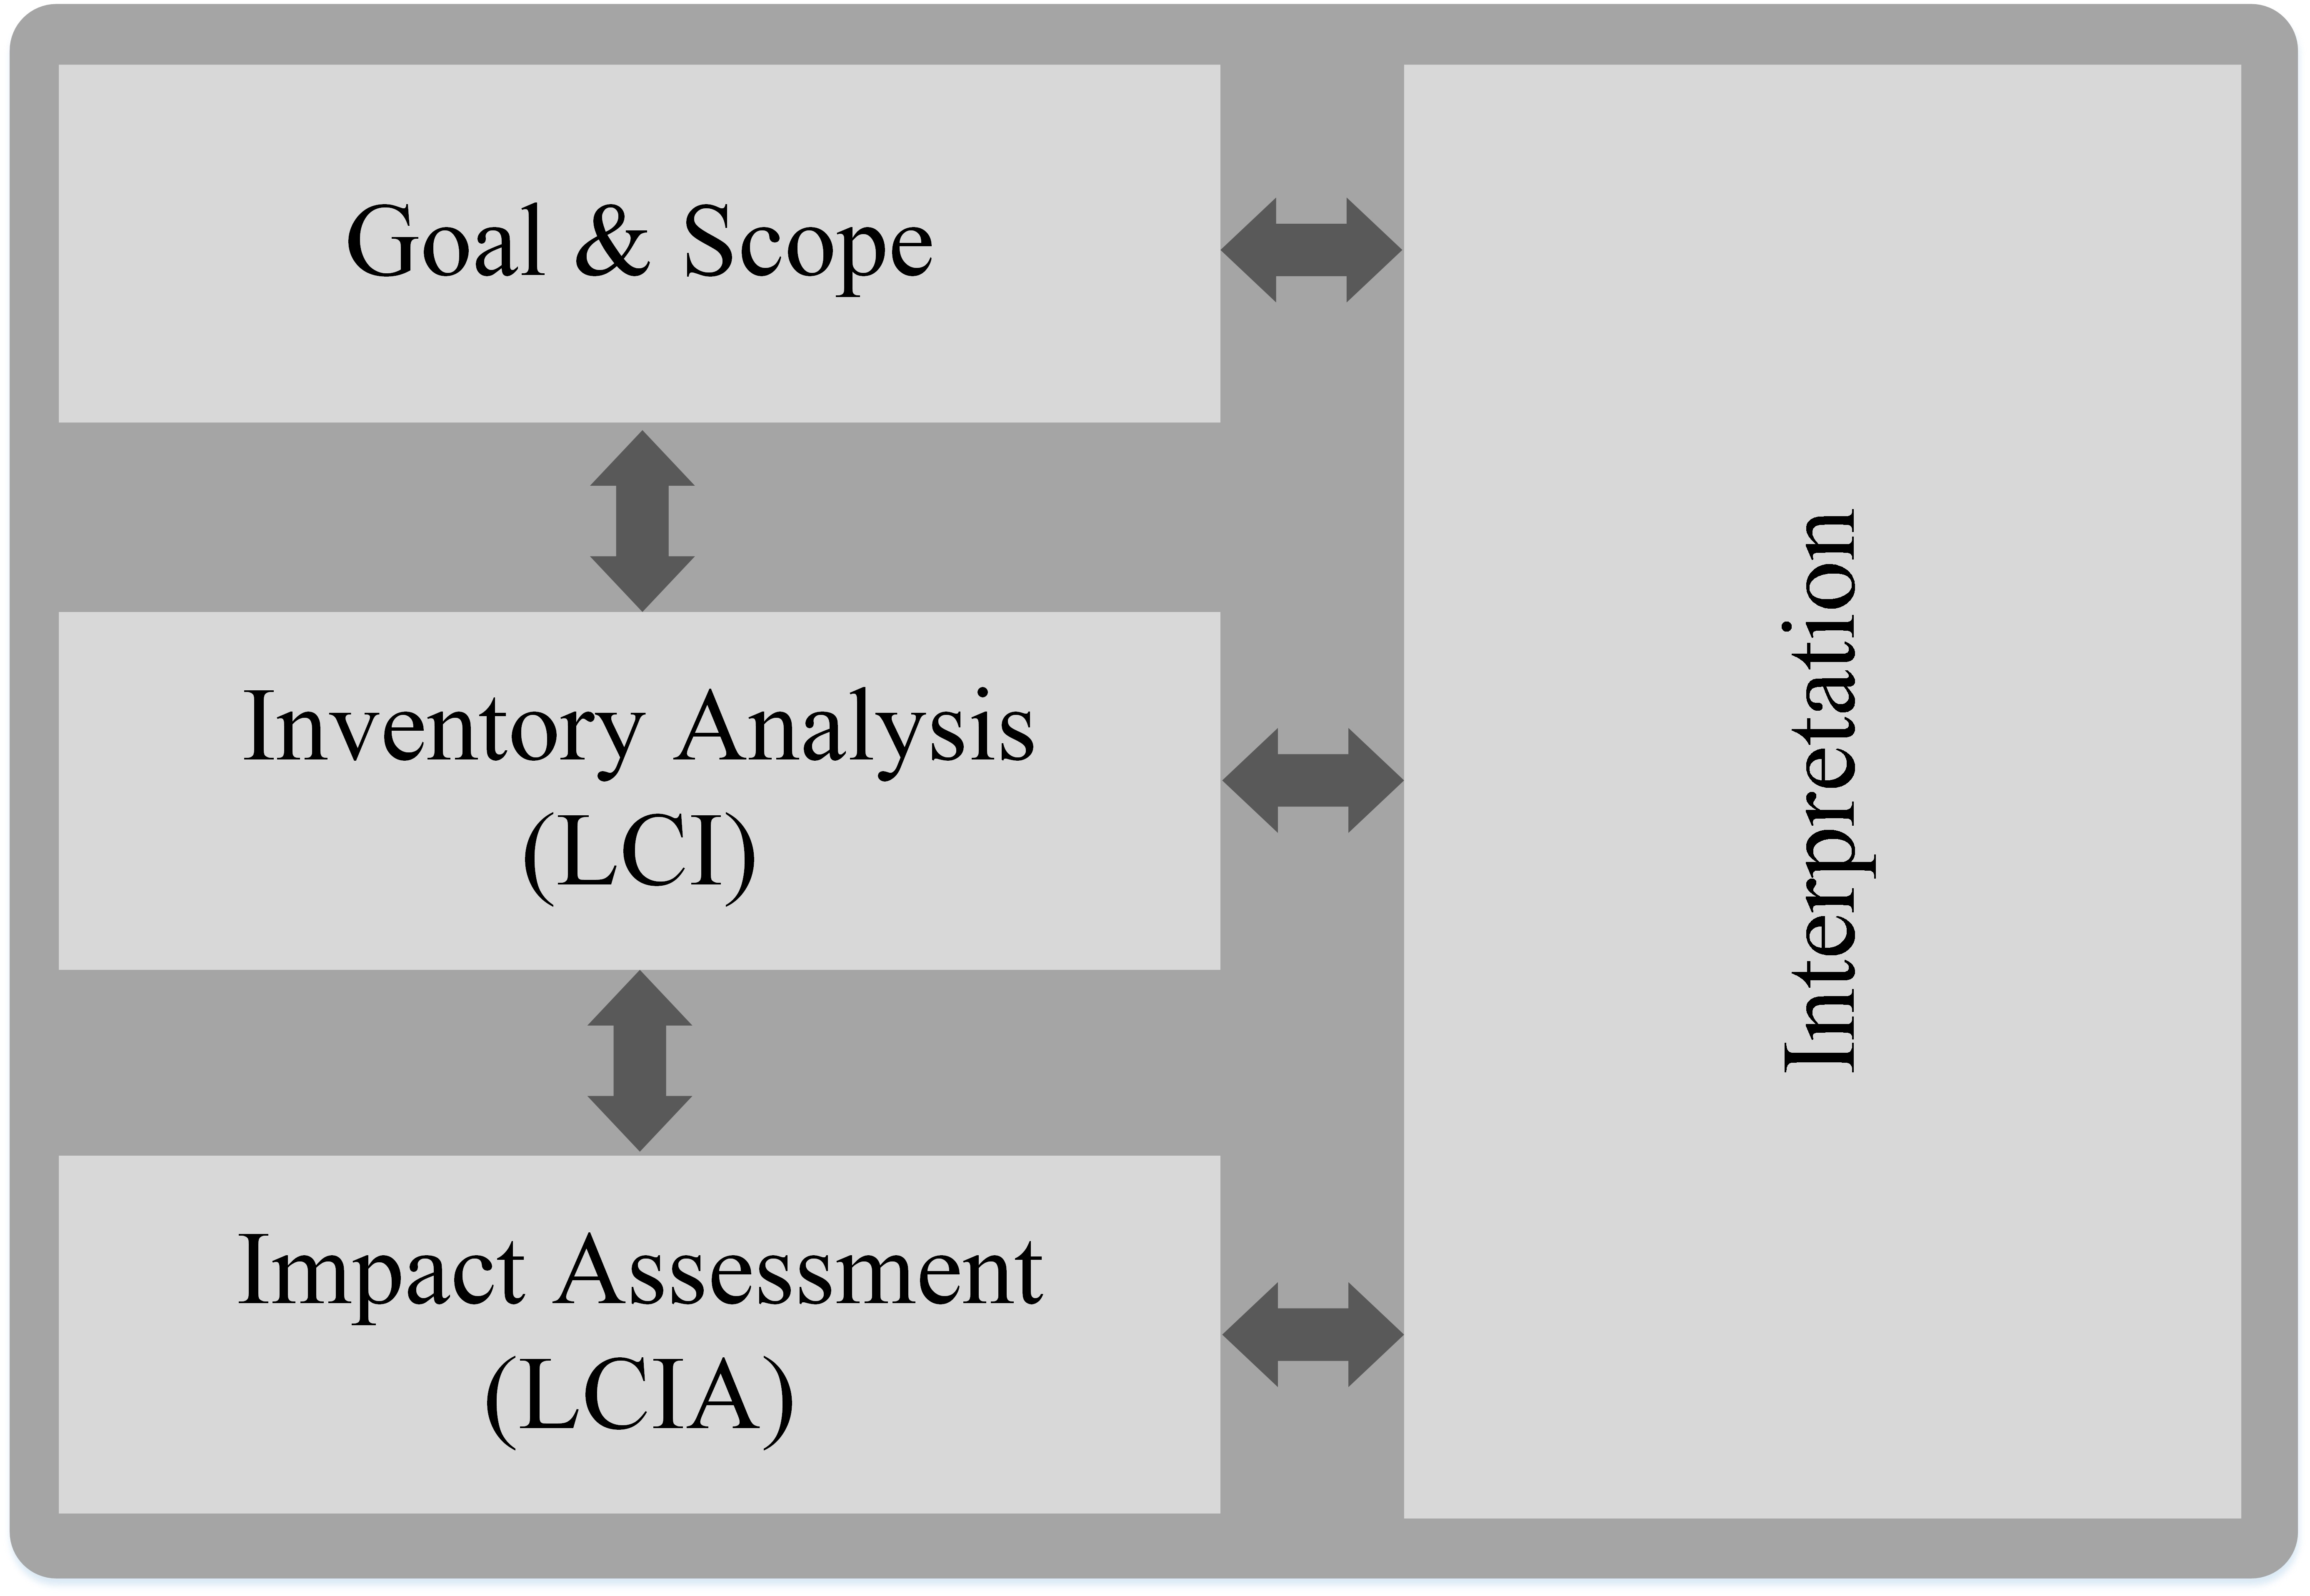
\includegraphics[width=0.4\columnwidth ]{ChapterLCA/Images/LCA_Framework_v3.jpg}
	   %\vspace*{-8cm}
		\caption{\hl{Life} cycle assessment (LCA) steps according to ISO 14040, 14044, and 14067.}
	\label{LCA_Methodology}  %This figure has not been referred to within the text of the manuscript. Please cite Figure 1 before the image of Figure 1. %Authors: It has been referred now. 
\end{figure}


{\subsection {Goal and Scope} \label{goalscope}}
{The goal and scope definition of an LCA provides the intended application of the analysis, describes the product system boundaries, and defines the functional unit \cite{REBITZER2004701}, determining and guiding the choices to be made in other stages of the analysis. Table \ref{screeninglca} defines the goal and scope for this study.} {In this article, the attributional LCA approach was applied for peak hours, developing a new LCA methodology named peak-hourly life cycle assessment (PH-LCA). As a result of this study, comparison between the environmental impacts of average and peak-hours  electricity produced in an entire year can be analyzed.} 

{The functional unit for the environmental impact assessment is defined as one kWh of electricity produced and delivered to the grid, which is in line with previous studies of the environmental impacts of electricity generation \cite{Nilsson2017AssessingEmissions, Khan2018, Khan2018AnalysisIntensity, MESSAGIE2014469, Cubi2015IncorporationAssessment, Buyle2019}. The impact category chosen for the assessment was global warming potential (GWP), using the CML 2015 life cycle impact assessment method \cite{Guinee2001}.} 

%%%%%%%%%%%%%% SCREENING TABLE %%%%%%%%%%%%%%%%%%%%%%%%%%%%

\begin{table}[]
\label{screeninglca}
\caption{Electricity grid mix LCA goal and scope structure.}
\resizebox{\textwidth}{!}{%
\begin{tabular}{lll}
\toprule
%%\multicolumn{3}{|c|}{\textbf{Electricity grid mixes LCA}}                                                                                                                                                                                               %%\\ \hline
\multirow{4}{*}{\begin{turn}{90}\textbf{Goal}\hspace{8mm} \end{turn}}  & \textbf{Intended Application}      & Explorative study                                                                                                                                                                          \\ \cline{2-3} 
                                & \textbf{LCA Typology}         & Attributional LCA                                                                             \\ \cline{2-3} 
                                & \textbf{Purpose of the Study}      & \begin{tabular}[c]{@{}l@{}}Provide the reader knowledge to understand the environmental\\ impacts of peak hours' electricity production\end{tabular}                                  

\\ \cline{2-3} 
                                & \textbf{Comparative Analysis}      & \begin{tabular}[c]{@{}l@{}}This is not a comparative analysis between countries.\\Comparison between average and {peak-hourly} (PH)%Confirm the definition. CONFIRMED
~global warming potential (GWP) values. \end{tabular} \\ \hline

\multirow{8}{*}{\begin{turn}{90}\textbf{Scope}\hspace{5mm}\end{turn}} & \textbf{Function of the System}    & \begin{tabular}[c]{@{}l@{}}The targeted country's electricity grid mixes are in charge of\\ producing the electricity needed to meet the national load\\ in any instant\end{tabular}        \\ \cline{2-3} 
                                & \textbf{Functional Unit}           & 1 kWh \cite{Nilsson2017AssessingEmissions,Khan2018,Khan2018AnalysisIntensity}                                                                                                                                               \\ \cline{2-3} 
                                & \textbf{Reference Flow}            & Energy flow (kWh) of electricity                                                                                                                                                     \\ \cline{2-3} 
                                & \textbf{Description of the System} & \begin{tabular}[c]{@{}l@{}} {Bulgaria, Germany, The Netherlands, Norway, and Spain (Section \ref{CaseStudy})} \end{tabular}                                                              \\ \cline{2-3} 
                                & \textbf{System Boundaries}         & Cradle to Gate                                                                                                                                                                  \\ \cline{2-3} 
                                & \textbf{Allocation Procedures}     & {Detailed in Section \ref{SB}}                                                                                                                                          \\ \cline{2-3} 
                                & \textbf{Impact Assessment Method}  & \begin{tabular}[c]{@{}l@{}}CML 2015 \cite{Guinee2001}. Impact category : GWP {(}kg CO\textsubscript2-eq/kWh{)}\end{tabular}                                               %Please check the unit format and unify all. DONE, there were some errors alongside the text.  kg CO\textsubscript2\hl{-eq/kWh}
                                
                                \\ \cline{2-3} 
                                & \textbf{Data Requirements}         & Secondary data provided by ENTSO-E Transparency Platform                                                                                                                   \\ \bottomrule
  \end{tabular}                              
\label{screeninglca}
}
\end{table}


\subsubsection{System Boundaries} \label{SB}
The system boundaries limit the LCA framework by defining the resource inputs and the emissions outputs of the system, excluding those that are out of the LCA's scope. The included limitations should derive from the available hourly data from the statistical source used for the analysis (in this research, the ENTSO-E TP). Soimakallio et al. \cite{Soimakallio2011} describe the challenges of performing an LCA about electricity mixes, suggesting the main factors and variables to consider as system boundaries. Elements such as grid losses, electricity import/export, power plant consumption, and environmental impact allocation procedures are described in the following subsections. 

\subsection*{Grid Losses} 
Specifically in this LCA, the background system includes all the previous steps of the final electricity production process, like the extraction of the fuel, its refinement, and its transportation to the power plant. The foreground system is related to the effective production of 1 kWh inside the power plant. For the background system, the software tool dataset used for this research includes imported electricity from neighboring countries and transmission/distribution losses (e.g., the electricity mix of the country which exports the fuel, the losses in transportation, etc.). However, the foreground system does not include the same values, meaning that it does not contain the exports of the produced electricity in other countries, the imports of electricity from bordering nations, or the grid losses to distribute the produced electricity~\cite{PEInternational2014GaBiV6}. According to \cite{Soimakallio2011}, the difficulties in how  grid losses should be allocated between high-, medium-, and low-voltage consumers make the process excessively complicated for the losses contribution in the final results, especially in terms of GHG emissions. This is why grid losses (distribution, transmission) of the targeted countries are not considered in this model. Contrariwise, transformation losses are part of the model because these values can estimated through the efficiency of the power plants. 

\subsection*{Import/Export}
Another subject of discussion is the amounts of imported and exported  electricity from neighboring countries, as mentioned in the previous subsection. In ENTSO-E TP, the classification named \textit{Actual Generation per Production Type} includes the natural resources used for the electricity production, and refers to the amount of fuels utilized including the import of these substances from other countries. However, it does not include the already-produced electricity imports between bordering countries. These data are integrated in a different class in the ENTSO-E TP platform, as \textit{cross-border physical flows}, which is not taken into account in this study. In fact, incorporating electricity imports and exports in a national grid mix could lead to inaccuracy and imprecision when dealing with GWP calculations, because it is not possible to know from which power plants the electricity comes from. As a result, the analysis of Nillson et al. in \cite{Nilsson2017AssessingEmissions}, which contains Swedish electricity imports, could include minor defects compared to a baseline where exchanges are not considered. Considering only the geographical borders avoids any possible misconception, as was also done by Khan \cite{Khan2018}. Cubi et al. \cite{Cubi2015IncorporationAssessment} do not specify if imports and exports were counted, and Khan et al. \cite{Khan2018AnalysisIntensity} did not include them. Furthermore, in a recent paper by Moro et al. \cite{Moro2017}, four out of five targeted countries of this study (Bulgaria, Germany, Spain, and the Netherlands) had a very low carbon intensity variation of the electricity production after trading with other countries ($-$2\%, +2\%, $-$6\%, and $-$1\% respectively).



\subsection*{Power Plants{'}%Confirm the deletion of " Own". 
%authors: confirmed
~Consumption}
Regarding {the electricity consumption of power plants themselves}%power plants own electricity consumption values
%authors: confirmed 
, these values were taken from the official statistics of the IEA (International Energy Agency) through the LCA software tool, and so they were included in the model \cite{PEInternational2014GaBiV6}. Specifically, the power consumed in pumping the water in hydro pumped storage (PHS) power plants was considered when data from TP were available. The sources of electricity for the pumps were assessed according to the average national electricity mix presented in this study.

\subsection*{Combined Heat and Power Plant Emission Allocation Procedures}
Finding the suitable allocation factor can sometimes be problematic, and can have a significant impact on the LCA results. According to \cite{2006ISOGuidelines}, allocation should be avoided whenever possible. Combined heat and power plants (CHP) produce two outputs, and so it is necessary to allocate the environmental impacts of just the electricity production. LCA software tools present a database for every resource used in CHP power plants, such as natural gas, biogas, heavy fuel oil, hard coal, lignite, and biomass. In the used database, there are data regarding the share of electricity, the overall efficiency, and the share of electricity to thermal energy within a CHP plant. According to the description of the dataset, for the CHP production, allocation by exergetic content is considered. Whenever there seemed to be a lack of data regarding the amount of produced heat or the efficiency of CHP plants in a country's database, the research found that this was due to the low percentage of produced heat relative to the total energy originated, which was rounded down to 0.0 since it is usually only about 0.01 \cite{PEInternational2014GaBiV6}. Therefore, the allocation of CHP plants was considered as a part of the analysis only when data were available (Bulgaria, Germany, and the Netherlands).



%%%%%%%%%%%%%%% ENTSO-E. LCI %%%%%%%%%%%%%%%%%%%%%%%
\subsection {Life Cycle Inventory (LCI)} \label{LCI}


{LCI can be understood as a model of the product system which fulfills a function that is quantified in the functional unit. It requires hypothesis definition, data collection, and data modeling, resulting in an inventory table with all the environmental interventions. The objective of the LCI is to quantify the resources used and the emissions and waste per functional unit \cite{REBITZER2004701}. Traditional LCA approaches quantify the resources, emissions, and wastes on average per functional unit. However, when the aim is to quantify the environmental impacts on peak hours to develop flexibility services, this approach is not enough. The time variability of the electricity production is a fundamental issue to consider in order to correctly assess the GWP during different time slots. To achieve that objective, a new methodology named peak-hourly LCA is defined in Figure \ref{Methodology}, and it is compared to the traditional approach of LCA for electricity production.}

%\textcolor{cyan}{explicar pas a pas la metodologia. part fabio}

%\subsubsection{Methodology for Peak-hourly LCI}
%%%%%%%%%%%%%% METHODOLOGY FIGURE %%%%%%%%%%%%%%%%%%%%%%%%%

\begin{figure}[]
	\centering
	\includegraphics[width=0.7\columnwidth ]{ChapterLCA/Images/Methodology_visio_new_v5.jpg}
	   %\vspace*{-8cm}
		\caption{LCA methodology for peak hours electricity generation.}%Check if round brackets can be used instead of square ones to declare units.
	\label{Methodology}
\end{figure}

%%%%%%%%%%%%%%%%%%%%%%%%%%%%%%%%%%%%%%%%%%

{The methodology followed for this study is based on the identification of electricity production peak hours for every day of the year, compared to the base load.} Every single peak hour, {extracted from a statistical source}, was analyzed to define the resources used to meet the greatest electricity demand of the day. The electricity mix was normalized into the functional unit of 1 kWh. Then, the resultant GHG emissions, and therefore the GWP impact indicator values, were calculated. To compare the obtained results for peak-hours to average values, the traditional LCA approach was also implemented. In this case, all the hours of the year 2018 were considered. Accordingly, peak hours GWP values were compared with the average, resulting in monthly results to highlight the seasonal variations. 

{The scope of this comparison is based on individuating the differences in the use of various resources to meet the electricity demand in different time frames}.  A similar approach is followed in \cite{Khan2018, Khan2018AnalysisIntensity, Cubi2015IncorporationAssessment}, but the results are presented in order to show the link between electricity demand and carbon intensity and not to compare peak hour values with a fixed average. In \cite{Nilsson2017AssessingEmissions}, the aim is to determine the hourly time slot where the highest CO\textsubscript2 intensity takes place throughout the year. This approach may hide the seasonality between summer and winter, since the peak hour time slot differs from season to season. In this paper, the hourly analysis enhances the differentiation of GHG emissions from peak hours and off-peak hours. 

%\textcolor{cyan}{quines bases de dades fem servir nosaltres?}
This paper bases its results on the data extracted from the Transparency Platform (TP) of the European Network of Transmission System Operators for Electricity (ENTSO-E), as well as the GaBi\textsuperscript{\textregistered} Software database. {The software allows the carbon intensity of every source to be assessed, considering the electricity produced as input. The related database is essential to differentiate the impact of each technology in different nations, having variable country-based data in which the same power plant can have different emission factors according to the country in which it is based}.
 
The ENTSO-E TP database is based on hourly time periods. Hence, it is possible to determine the time slots where peak consumption takes place. A critical review of the ENTSO-E TP from 2018 in \cite{Hirth2018ThePlatform} points out a number of simplifications, but at the same time the review highlights that it is the single most important data source for European researchers. For this study the consistency of the data is guaranteed, supported by the fact they were compared, when possible, with the statistics from each national Transmission System Operator (TSO). As a result, the most complete and available data were used for the analysis, referring to the entire year 2018.  %This online data platform includes various electricity data, mainly reported by country or bidding zone. The data used for this study come from the sections \textit{Installed Capacity per Production Type} and \textit{Actual Generation per Production Type} and they are shared directly from the primary data owners, as TSOs or generator companies.
%To develop the GHG emission assessment model, based on LCA framework and considering both peak and off-peak hours from the ENTSO-E TP, the methodology presented in Figure \ref{Methodology} is applied, thanks to

%Thanks to the hourly data provided by the TP, it is possible to find out when peak hours occur and which resources are used during those times. 


%\textcolor{cyan}{Possibilitat de treure el títol i simplement posar-ho a continuació de l'explicació de la base de dades ENTSO-E}

%\subsection{LCA Methodology applied to targeted electricity grid mixes} 

The databases available for the development of electricity grid mixes analysis have limitations that hinder the accurate development of the model. For this reason, certain assumptions and hypotheses were considered. Even if from the ENTSO-E TP, the data for hydro production are divided into categories such as {hydro pumped storage, hydro run-of-river and poundage, and hydro water reservoir;%Confirm the removal of capitalizations.
%authors: confirmed
~these were all merged together in this work. {The reference value for hydro power plants is the carbon intensity provided by the database, which makes a mean between the different types of hydro technologies}. The same procedure was used to calculate the environmental impacts of wind power production, {grouping}%putting together. confirmed
~onshore and offshore wind only for Germany and the Netherlands (the two countries which have both technologies). ENTSO-E shows data including solar thermal and solar photovoltaic electricity in the same box (i.e., \textit{Solar}), without any distinction. Thus, the model was developed incorporating the data in the Electricity from photovoltaics%Are the italics necessary? Check that consistent notation is used throughout the paper. (e.g., should "hydro run-of-river" also be italicized?)
%authors: No, italics are not required here. They can be removed 
~GaBi\textsuperscript{\textregistered} Software model.


%% GaBi \\
%The LCA model detailed in this paper is implemented by means of GaBi Software. The GaBi database includes countries' specific data about electricity production which allow to perform a country based analysis underlining the environmental impact differences. For example, the production of 1 kWh from a hard coal power plant based in Germany has a different output compared with the same typology in Bulgaria; 1.01 kg CO\textsubscript2\textsubscript e\textsubscript q\textsubscript./kWh in Germany and 1.28 kg CO\textsubscript2\textsubscript e\textsubscript q\textsubscript./kWh in Bulgaria.  \\

{\subsection{Life Cycle Impact Assessment (LCIA)}}
{Life cycle impact assessment (LCIA) yields indicators  that evaluate the product life cycle on a functional unit basis, considering one or several impact categories. For the purpose of this study, the impact category used to assess the potential environmental impact of the electricity production was the global warming potential, measured in kg CO\textsubscript2-eq/kWh}. Section \ref{CaseStudy} provides the results of the LCIA stage.}

\section{Case Study: INVADE H2020 Project Pilot-Sites Electricity Grid Mixes} \label{CaseStudy}
\subsection{INVADE Project Description}

The methodology described in Section \ref{Methodology_text} was applied under the H2020 INVADE project to assess the potential environmental impact of large-scale pilots integrating DERs and EVs, by means of a cloud-based platform for {the provision of flexibility services}%was "flexibility services providing", confirm that your intended meaning is retained.%authors: it should be flexibility, and not flexible, since the service to be provided is flexibility and not flexible. 
. Denominated \textit{Integrated electric vehicles and batteries to empower distributed and centralized storage in distribution grids}, this project belongs to the  \textit{Low-Carbon Energy} call of the Horizon 2020 Work Program 2016--2017. This project is based on five pilot sites located in five different countries, which are  environmentally assessed in the following section.  %The main focus is to design a flexibility management system that enhances the integration of  supports the distribution grid and electricity market while coping with grid limitations, uncertainty and variability with high penetration of renewable energy, electric vehicles and an increased number of diverse smart grid actors. To provide these services, the INVADE Platform is based on a flexibility cloud that enables flexibility operations to be provided by means of decision-making algorithms, functions and control dashboards using Internet of Energy Things, Artificial Intelligence and Big Data analytics.
%It is worth noting that the integration of distributed generation as well as electric vehicles and storage may change the total electricity production and consumption patterns. Therefore, it can lead to a change in the potential environmental impacts of the energy system, being this the main objective of the LCA task in the INVADE project.\\

\subsection{Overview of the Installed Capacity of Pilot Site Countries} 

The installed capacity represents the total amount of power in MW that is installed in a country. It determines the  resources the country has available to meet the demand, representing the {number}%amount
~of power plants that can be used for electricity generation in a targeted country. 
As can be seen in  Table \ref{table:capacity}, the targeted countries of the H2020 INVADE project have different  installed capacities. These data represent the percentage of power plants which can produce electricity in the country divided by source used, and are not directly related to the power generation. For example, in Spain the maximum hourly power request in 2018 was 42 GW, but the country has nearly 105 GW of installed capacity. This means that even if the power plants which are run by natural gas represent the major share of the installed capacity (29.3\%), it does not necessarily{ mean that}%was "coincide with", confirm that your meaning is retained. %authors: Yes, confirmed
~the highest share of electricity production in 2018 was from natural gas, as determined in Section \ref{LCIA}.
% \begin{table}[htbp]
% \caption{Electricity installed capacity in the targeted countries for the year 2018}
% \begin{tabular}{l|c|c|c|}
% \cline{2-4}

%                                           & \textbf{Main}                                                                                             & \textbf{Flexible hydro power}                                                         & \textbf{Others}                                                                                                    \\ \hline
% \multicolumn{1}{|l|}{\textbf{Bulgaria}}    & \begin{tabular}[c]{@{}c@{}}Lignite (33.3\%), Hydro (25.2\%), \\ Nuclear (15\%)\end{tabular}               & \begin{tabular}[c]{@{}c@{}}Pumped storage (6.8\%),\\ Reservoir (14.2\%)\end{tabular}  & \begin{tabular}[c]{@{}c@{}}Solar (8.2\%), Natural Gas (6.1\%),\\ Wind onshore (5.5\%), Others (5.8\%)\end{tabular} \\ \hline
% \multicolumn{1}{|l|}{\textbf{Germany}}     & \begin{tabular}[c]{@{}c@{}}Wind (26.6\%), Solar (19.6\%),\\ Natural Gas (14.3\%)\end{tabular}             & \begin{tabular}[c]{@{}c@{}}Pumped storage (4.2\%),\\ Reservoir (0.5\%)\end{tabular}   & \begin{tabular}[c]{@{}c@{}}Hard coal (11.4\%), Lignite (9.6\%), \\ Hydro (6.5\%), Others (12\%)\end{tabular}       \\ \hline
% \multicolumn{1}{|l|}{\textbf{Netherlands}} & \begin{tabular}[c]{@{}c@{}}Natural Gas (57.6\%), Hard coal (14.5\%),\\ Wind Onshore (11.5\%)\end{tabular} & \begin{tabular}[c]{@{}c@{}}Pumped storage (0\%),\\ Reservoir (0\%)\end{tabular}      & \begin{tabular}[c]{@{}c@{}}Solar (8.1\%), Wind Offshore (3\%),\\ Waste (2.1\%), Others (3.2\%)\end{tabular}        \\ \hline
% \multicolumn{1}{|l|}{\textbf{Norway}}      & \begin{tabular}[c]{@{}c@{}}Hydro (93.2\%), \\ Wind Onshore (3.5\%)\end{tabular}                           & \begin{tabular}[c]{@{}c@{}}Pumped storage (10.8\%),\\ Reservoir (78.5\%)\end{tabular} & Thermal power* (3.3\%)                                                                                             \\ \hline
% \multicolumn{1}{|l|}{\textbf{Spain}}       & \begin{tabular}[c]{@{}c@{}}Natural Gas (29.3\%), Hydro (24.7\%),\\ Wind Onshore (21.7\%)\end{tabular}     & \begin{tabular}[c]{@{}c@{}}Pumped storage (5.4\%),\\ Reservoir (18.22\%)\end{tabular} & \begin{tabular}[c]{@{}c@{}}Hard coal (9.1\%), Nuclear (6.8\%),\\ Solar (6.4\%), Others (2\%)\end{tabular}          \\ \hline
% \end{tabular}
%  \begin{tablenotes}
%   \vspace*{3mm}
%       \small
%       \item * Norway data are by \cite{Norway}
%     \end{tablenotes}
% \label{table:capacity}
% \end{table}



 \begin{table}[]
\caption{Electricity installed capacity in the targeted countries for the year 2018.}
\begin{tabular}{llll}
\toprule

                                           & \textbf{Main}                                                                                             & \textbf{Flexible Hydro Power}                                                         & \textbf{Others}                                                                                                    \\ \hline
\multicolumn{1}{l}{\textbf{Bulgaria }- (12,708 MW)}    & \begin{tabular}[l]{@{}l@{}}Lignite (33.7\%) \\Hydro (25.2\%) \\Nuclear (15.5\%)\end{tabular}               & \begin{tabular}[l]{@{}l@{}}Pumped storage (6.8\%)\\ Reservoir (14.2\%)\end{tabular}  & \begin{tabular}[l]{@{}l@{}}Solar (8.2\%)\\ Natural gas (6.1\%)\\ Wind onshore (5.5\%)\\ Others (5.8\%)\end{tabular} \\ \hline
\multicolumn{1}{l}{\textbf{Germany }- (221,020 MW)}     & \begin{tabular}[l]{@{}l@{}}Wind (26.6\%)\\Solar (19.6\%)\\ Natural gas (14.3\%)\end{tabular}             & \begin{tabular}[l]{@{}l@{}}Pumped storage (4.2\%)\\ Reservoir (0.5\%)\end{tabular}   & \begin{tabular}[l]{@{}l@{}}Hard coal (11.4\%)\\ Lignite (9.6\%) \\ Hydro (6.5\%) \\ Others (12\%)\end{tabular}       \\ \hline
\multicolumn{1}{l}{\textbf{Netherlands} - (30,531 MW)} & \begin{tabular}[l]{@{}l@{}}Natural gas (57.6\%)\\ Hard coal (14.5\%)\\ Wind Onshore (11.5\%)\end{tabular} & \begin{tabular}[l]{@{}l@{}}Pumped storage (0\%)\\ Reservoir (0\%)\end{tabular}      & \begin{tabular}[l]{@{}l@{}}Solar (8.1\%)\\ Wind Offshore (3\%)\\ Waste (2.1\%)\\ Others (3.2\%)\end{tabular}        \\ \hline
\multicolumn{1}{l}{\textbf{Norway }- (33,755 MW)}      & \begin{tabular}[l]{@{}l@{}}Hydro (93.2\%) \\ Wind Onshore (3.5\%)\end{tabular}                           & \begin{tabular}[l]{@{}l@{}}Pumped storage (10.8\%)\\ Reservoir (78.5\%)\end{tabular} & Thermal power* (3.3\%)                                                                                             \\ \hline
\multicolumn{1}{l}{\textbf{Spain} - (104,975 MW)}       & \begin{tabular}[l]{@{}l@{}}Natural gas (29.3\%)\\ Hydro (24.7\%)\\ Wind Onshore (21.7\%)\end{tabular}     & \begin{tabular}[l]{@{}l@{}}Pumped storage (5.4\%)\\ Reservoir (18.22\%)\end{tabular} & \begin{tabular}[l]{@{}l@{}}Hard coal (9.1\%)\\ Nuclear (6.8\%)\\ Solar (6.4\%)\\ Others (2\%)\end{tabular}          \\ \bottomrule
\end{tabular}\\


\begin{tabular}{@{}c@{}} 
\multicolumn{1}{p{\textwidth -.88in}}{\footnotesize {Source:} ENTSO-E TP \cite{Entso-eProduction}. * The installed capacity data from Norway in ENTSO-E TP were not sufficient. More detailed data come from  \cite{ssb2017StatisticsNorway}.}
\end{tabular}

% \begin{tablenotes}
%   \vspace*{3mm}
%      \small
%      \item Source: ENTSO-E TP \cite{Entso-eProduction}\\
%      *The installed capacity data from Norway in ENTSO-E TP are not sufficient. More detailed data come from  \cite{ssb2017StatisticsNorway}
%    \end{tablenotes}
\label{table:capacity}
\end{table}

\subsection{LCIA: GWP Results}
\label{LCIA}
%% other options for these titles: LCIA GWP results 
%% carbon footprint results 

This section presents the results of the performed LCA. As mentioned in Section \ref{LCI}, the GWP impact factors of each technology are dependent on the country they are based in. However, to frame the studied context, Table \ref{EmissionFactors} shows the average life cycle emission factors for electricity generation from the most used technologies in Europe, according to Turconi et al. \cite{Turconi2013LifeLimitations}.

The values in  Table \ref{EmissionFactors} include upstream and downstream processes and thus all the steps involved in the electricity generation, like the construction of the power plants and Operations and Maintenance (O\&M)%Define if appropriate. %authors: we have defined it.
~procedures. The ranges of the values are wide, because the 167 case studies analyzed have different system boundaries and methodologies \cite{Turconi2013LifeLimitations}. Even so, the software used in this study has a specific country-based database for each technology, conferring the results a significant precision. {As it is possible to see from Table \ref{EmissionFactors}, even renewable sources have non-zero GWP values. This is due to indirect emissions, especially related to the manufacturing of the components for the construction of renewable power plants, which are taken into account in this study.}  

 \begin{table}[]
\centering
\caption{Emission factors of power production technologies. Extracted from \cite{Turconi2013LifeLimitations}.}
\label{EmissionFactors}
\begin{tabular}{cc}
\toprule
\textbf{Energy Source} & \textbf{GWP} (kg CO\textsubscript2-eq/kWh{)} \\ \hline
Hard coal              & 0.66--1.05                   \\ 
Lignite                & 0.8--1.3                     \\
Natural gas, single cycle           & 0.61--0.85                    \\ 
Natural gas, combined cycle           & 0.36--0.59                    \\ 
Oil                    & 0.53--0.9                    \\ 
Nuclear                & 0.003--0.035                 \\ 
Biomass                & 0.008--0.13                  \\ 
Hydropower             & 0.002--0.02                  \\ 
Solar photovoltaic (PV)%Confirm the definition. Authors: CONFIRMED
                  & 0.013--0.19                  \\ 
Wind                   & 0.003--0.041                 \\ \bottomrule
\end{tabular}
\end{table}



Two types of graphs (Figures \ref{GWP_BG} -\ref{COMP_ES}), \textcolor{red}{area and line plots, are presented in the following sections to facilitate the comprehension of the results. Area \hl{plots}, represented by odd Figures \ref{GWP_BG}, \ref{GWP_DE}, \ref{GWP_NL}, \ref{GWP_NO}, \ref{GWP_ES}, 
~show the GWP value of each resource used only during peak hours in the related country's grid mix.} The outcomes are shown month by month and are compared with the average GWP value (represented by a dotted line), which takes into account all the hours of the year. This is why the dotted line does not coincide with the average of the values of the 12 months. % Please call out figures in order.Figure 5,7,9,11 was cited before Figure 6,8,10. Incorrect order. Please renumber Figures so they appear in sequence number. #Authors: we cannot change the order or renumber figures since they are per each country. Hence, we have changed the sentence in order to cite them in order and then group them according to the type of graph.  

However, it is possible that resources such as hydro and nuclear, even though they have a great share of the electricity production,  could not appear in the graph because of their low carbon impact factors (Table \ref{EmissionFactors}). \textcolor{red}{Line plots, represented by even Figures \ref{COMP_BG}, \ref{COMP_GE}, \ref{COMP_NL}, \ref{COMP_NO}, and \ref{COMP_ES};} correspond to the variation in the percentage of use of the most representative sources during the year, compared with the monthly peak hours GWP variations. {All the previous listed figures were made with our own calculations and estimations through MATLAB\textsuperscript{\textregistered}. All data sources have already been mentioned in the text, namely the  GaBi\textsuperscript{\textregistered} Software professional database and the ENTSO-E TP.} {Every energy source grouped under the label ``Others'' was calculated in terms of carbon intensity in the same way as the other main sources. Nevertheless, their weights were too low to be represented on the chosen plot typology, and for that reason the results are merged in a single and more general group}.\\





%%%%%%%%%%%%%%%%%%%%%%%%% BG %%%%%%%%%%%%%%%%%%%%%%%%%%%%%%%
\subsubsection{Bulgaria}
The electricity demand of this southeastern European country  during the year is mainly covered by lignite and nuclear power, as explained in Table \ref{RES_BG}. The high percentage of hydro power capacity (Table \ref{table:capacity}) is reflected in the  consistent use of hydro power plants. Solar and wind power together represented  just 5.35\% of the total electricity production in Bulgaria in 2018. The total electricity produced during the year was equal to 45.2 TWh. 
 
 
 \begin{table}[]
\centering
\caption{Percentage of resources used during peak and off-peak hours in Bulgaria  \cite{Entso-eProduction}.}
\label{RES_BG}
\begin{tabular}{ccccccc}
\toprule
\textbf{Lignite} &  \textbf{Nuclear} &  \textbf{Hydropower} & \textbf{Natural Gas} & \textbf{Wind} & \textbf{Solar} &  \textbf{Others} \\ \hline
42.29\% & 34.78\%  & 11.42\%  & 4.26\%             & 2.75\%  & 2.60\%    & 1.90\%          \\ \bottomrule
\end{tabular}
\end{table}
 
Consequently, the GWP during peak hours was mainly based on lignite (Figure \ref{GWP_BG}). The GWP during peak hours was higher than the average from September to December because of higher use of lignite and a lower use of flexible hydro to cover the peak demand {(+6.65\% more on average)}. From Figure  \ref{COMP_BG}, it is possible to see the direct correlation between the use of lignite and hydropower during peak hours and the GWP. Hydropower and lignite are the only two represented resources because they were the only ones with a significant variation in their usage throughout the year. When there was the possibility to use the hydro reservoirs and the hydro pumped storage, the GWP decreased in comparison with the average. The months in which the power production during peak hours was greater than the average showed higher values of GWP. The reason is that  nuclear power represents a huge and constant portion of the base production {(34.78\% throughout the year)}, and the less extra power is needed, the less fossil fuels are used to generate it. The two presented curves of lignite and hydro in Figure \ref{COMP_BG} have exactly the opposite trends. April is a symbolic month, with the highest share usage of hydro and the lowest of lignite,  leading to the lowest GWP of the year ({0.397 kg CO\textsubscript2-eq/kWh). The reasons behind this event are related to the low power production in April and possibly to the abundance of water resources. 
 
\begin{figure}[]
	\centering
	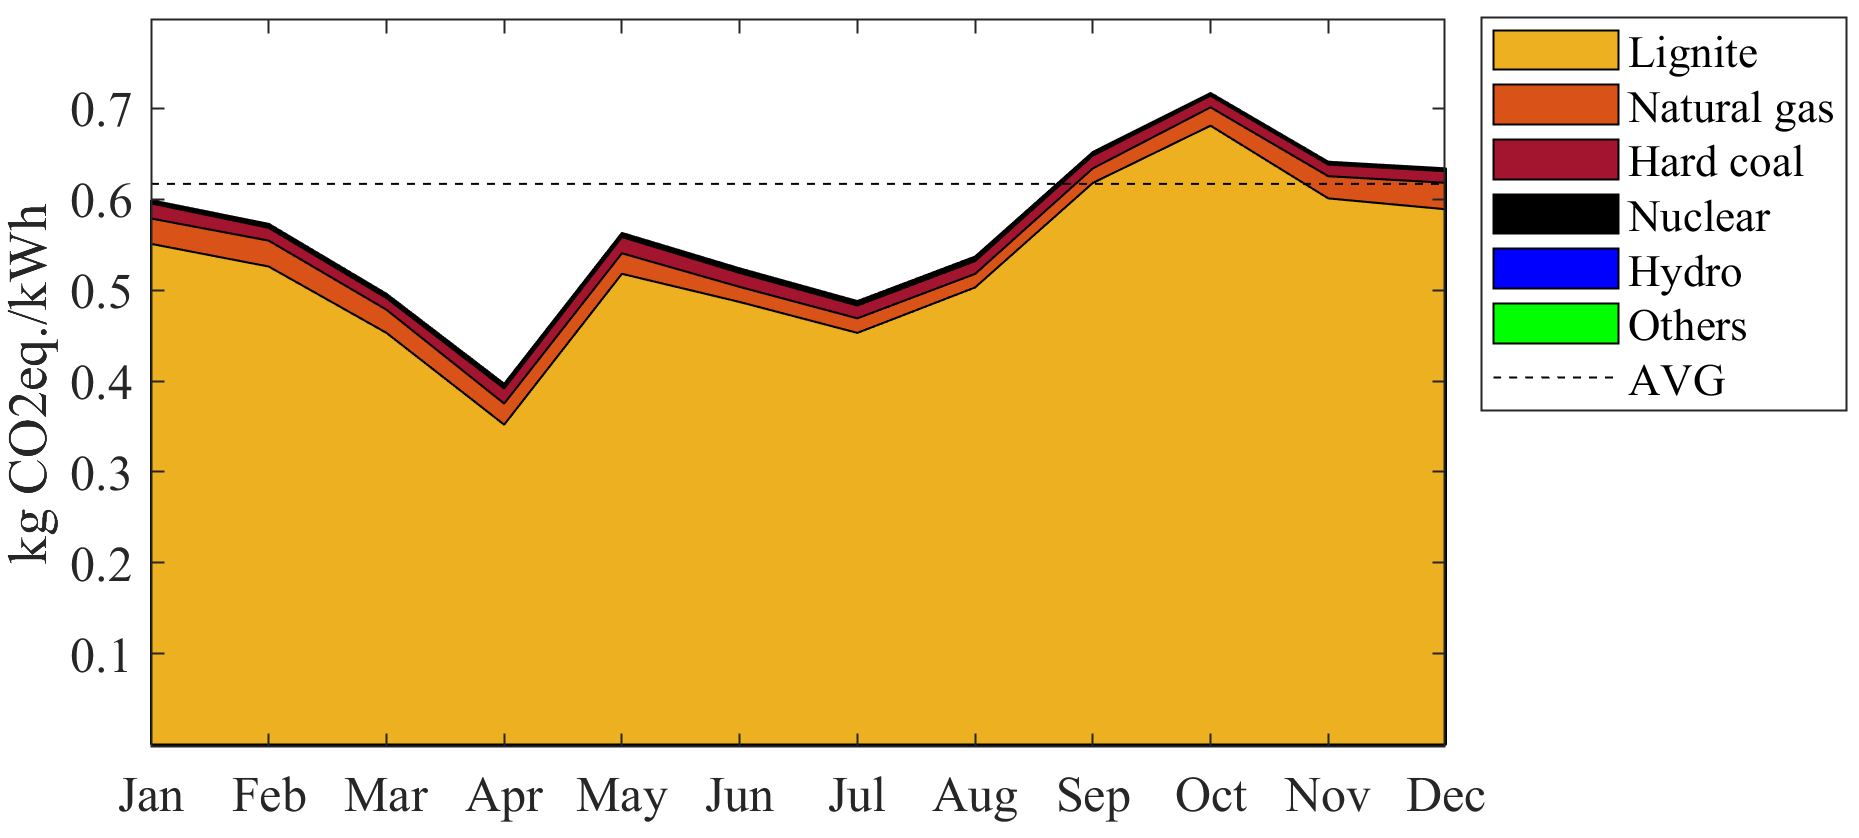
\includegraphics[width=1\textwidth]{ChapterLCA/Images/GWP_plots/Bulgaria_GWP.png}
   \vspace*{-15mm}
\hspace*{-1cm}	\caption{Monthly peak hours GWP compared with average through the year (dotted line) in Bulgaria.}
	\label{GWP_BG}
\end{figure} 
	\vspace*{-7mm}
\begin{figure}[]
	\centering
	\hspace*{0.2cm}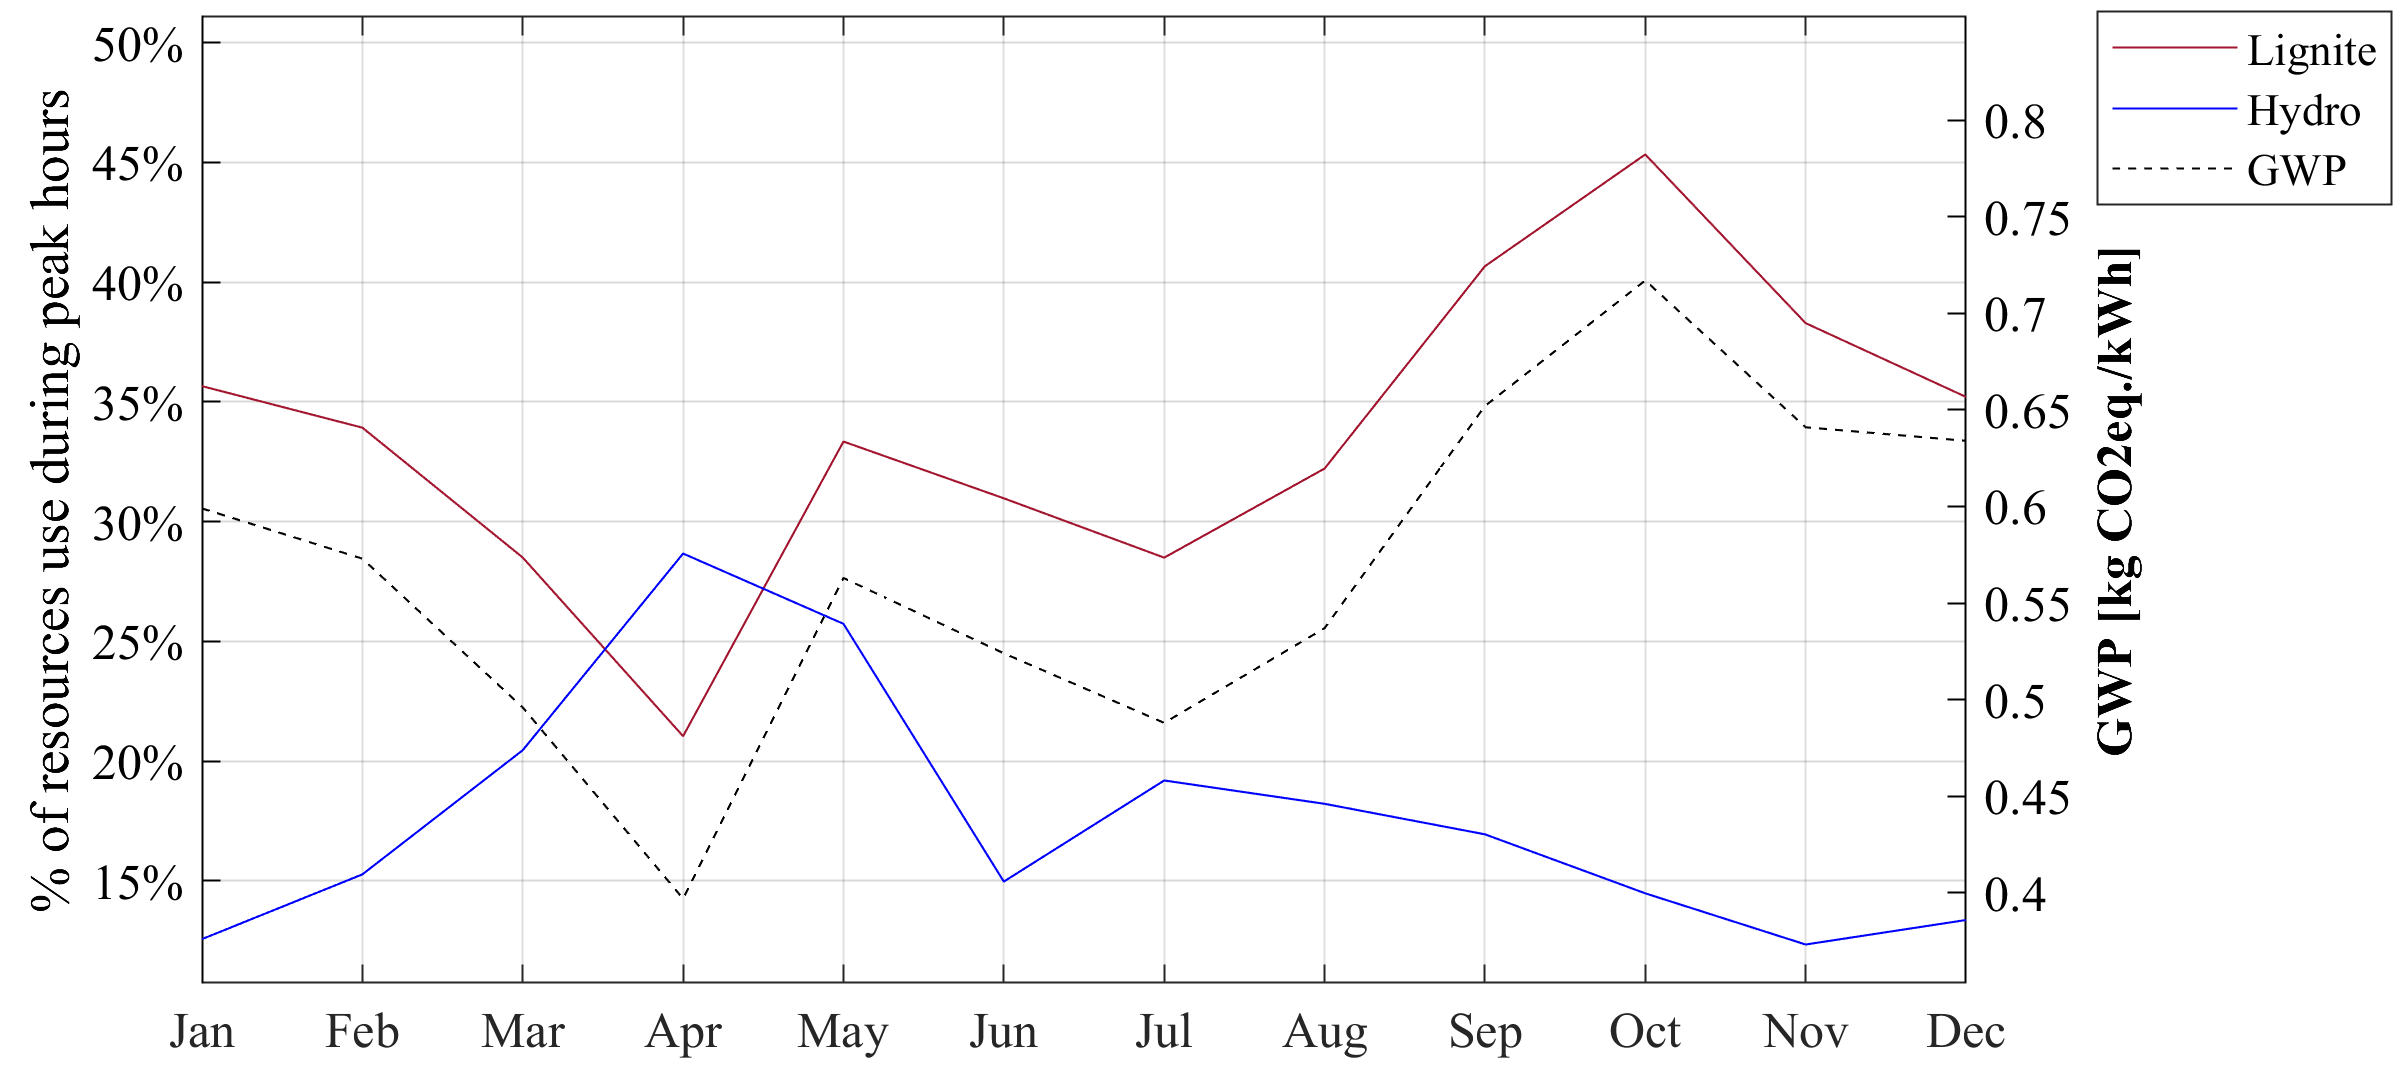
\includegraphics[width=1.2\textwidth]{ChapterLCA/Images/GWP_plots/Comp_GWP_BG.png}
	\vspace*{-20mm}
\hspace*{-1cm}	\caption{Percentage use of resources throughout the year compared with monthly GWP in Bulgaria, both related to peak hours.}
	\label{COMP_BG}
\end{figure}






%%%%%%%%%%%%%%%%%%%%%%%%% DE %%%%%%%%%%%%%%%%%%%%%%%%%%%%%%%
\subsubsection{Germany}
Germany has a national production mix which relies on different sources. Regarding the base load, lignite and hard coal, {respectively 24.46\% and 13.72\%,} were the most used fossil fuels. The use of lignite throughout 2018 was almost constant, as shown in Figure \ref{GWP_DE}. Wind farms had the highest share of capacity in the country and a total share of production of 20.63\%, as presented in Table \ref{table:capacity} and Table \ref{RES_DE}. Nuclear still had  a regular contribution {(13.64\%)}, while solar {(7.83\%)} and biomass {(7.63\%)} power plants surpassed the use of natural gas {(6.41\%)} in 2018. Hydropower accounted for just 2.81\% of the total electricity production. The total electricity produced during the year in the country was equal to 2183.6 TWh. 


 \begin{table}[]
\centering
\caption{Percentage of resources used during peak and off-peak hours in Germany \cite{Entso-eProduction}.}
\label{RES_DE}
\resizebox{\textwidth}{!}{%
\begin{tabular}{ccccccccc}
\toprule
 \textbf{Lignite}& \textbf{Wind} & \textbf{Hard Coal}& \textbf{Nuclear} & \textbf{Solar}    & \textbf{Biomass} & \textbf{Natural Gas}  & \textbf{Hydro}  & \textbf{Others*} \\ \hline
 24.42\%    & 20.63\%   & 13.72\%  & 13.64\%   & 7.83\%  & 7.63\%           &     6.41\%                         & 2.81\%                             & 2.91\%                         \\ \bottomrule
\end{tabular}%
}
% \begin{tablenotes}
%   \vspace*{2mm}
%      \small
%      \item *Others includes: coal gas derived,  fossil oil, geothermal, other renewables, waste
%    \end{tablenotes}
\begin{tabular}{@{}c@{}} 
\multicolumn{1}{p{\textwidth -.88in}}{\footnotesize {*Others} includes: coal gas derived,  fossil oil, geothermal, other renewables, waste.}
%    \end{tablenotes}
\end{tabular}
\end{table}

\vspace{-8mm}

\begin{figure}[]
	\centering
	\hspace*{-1cm}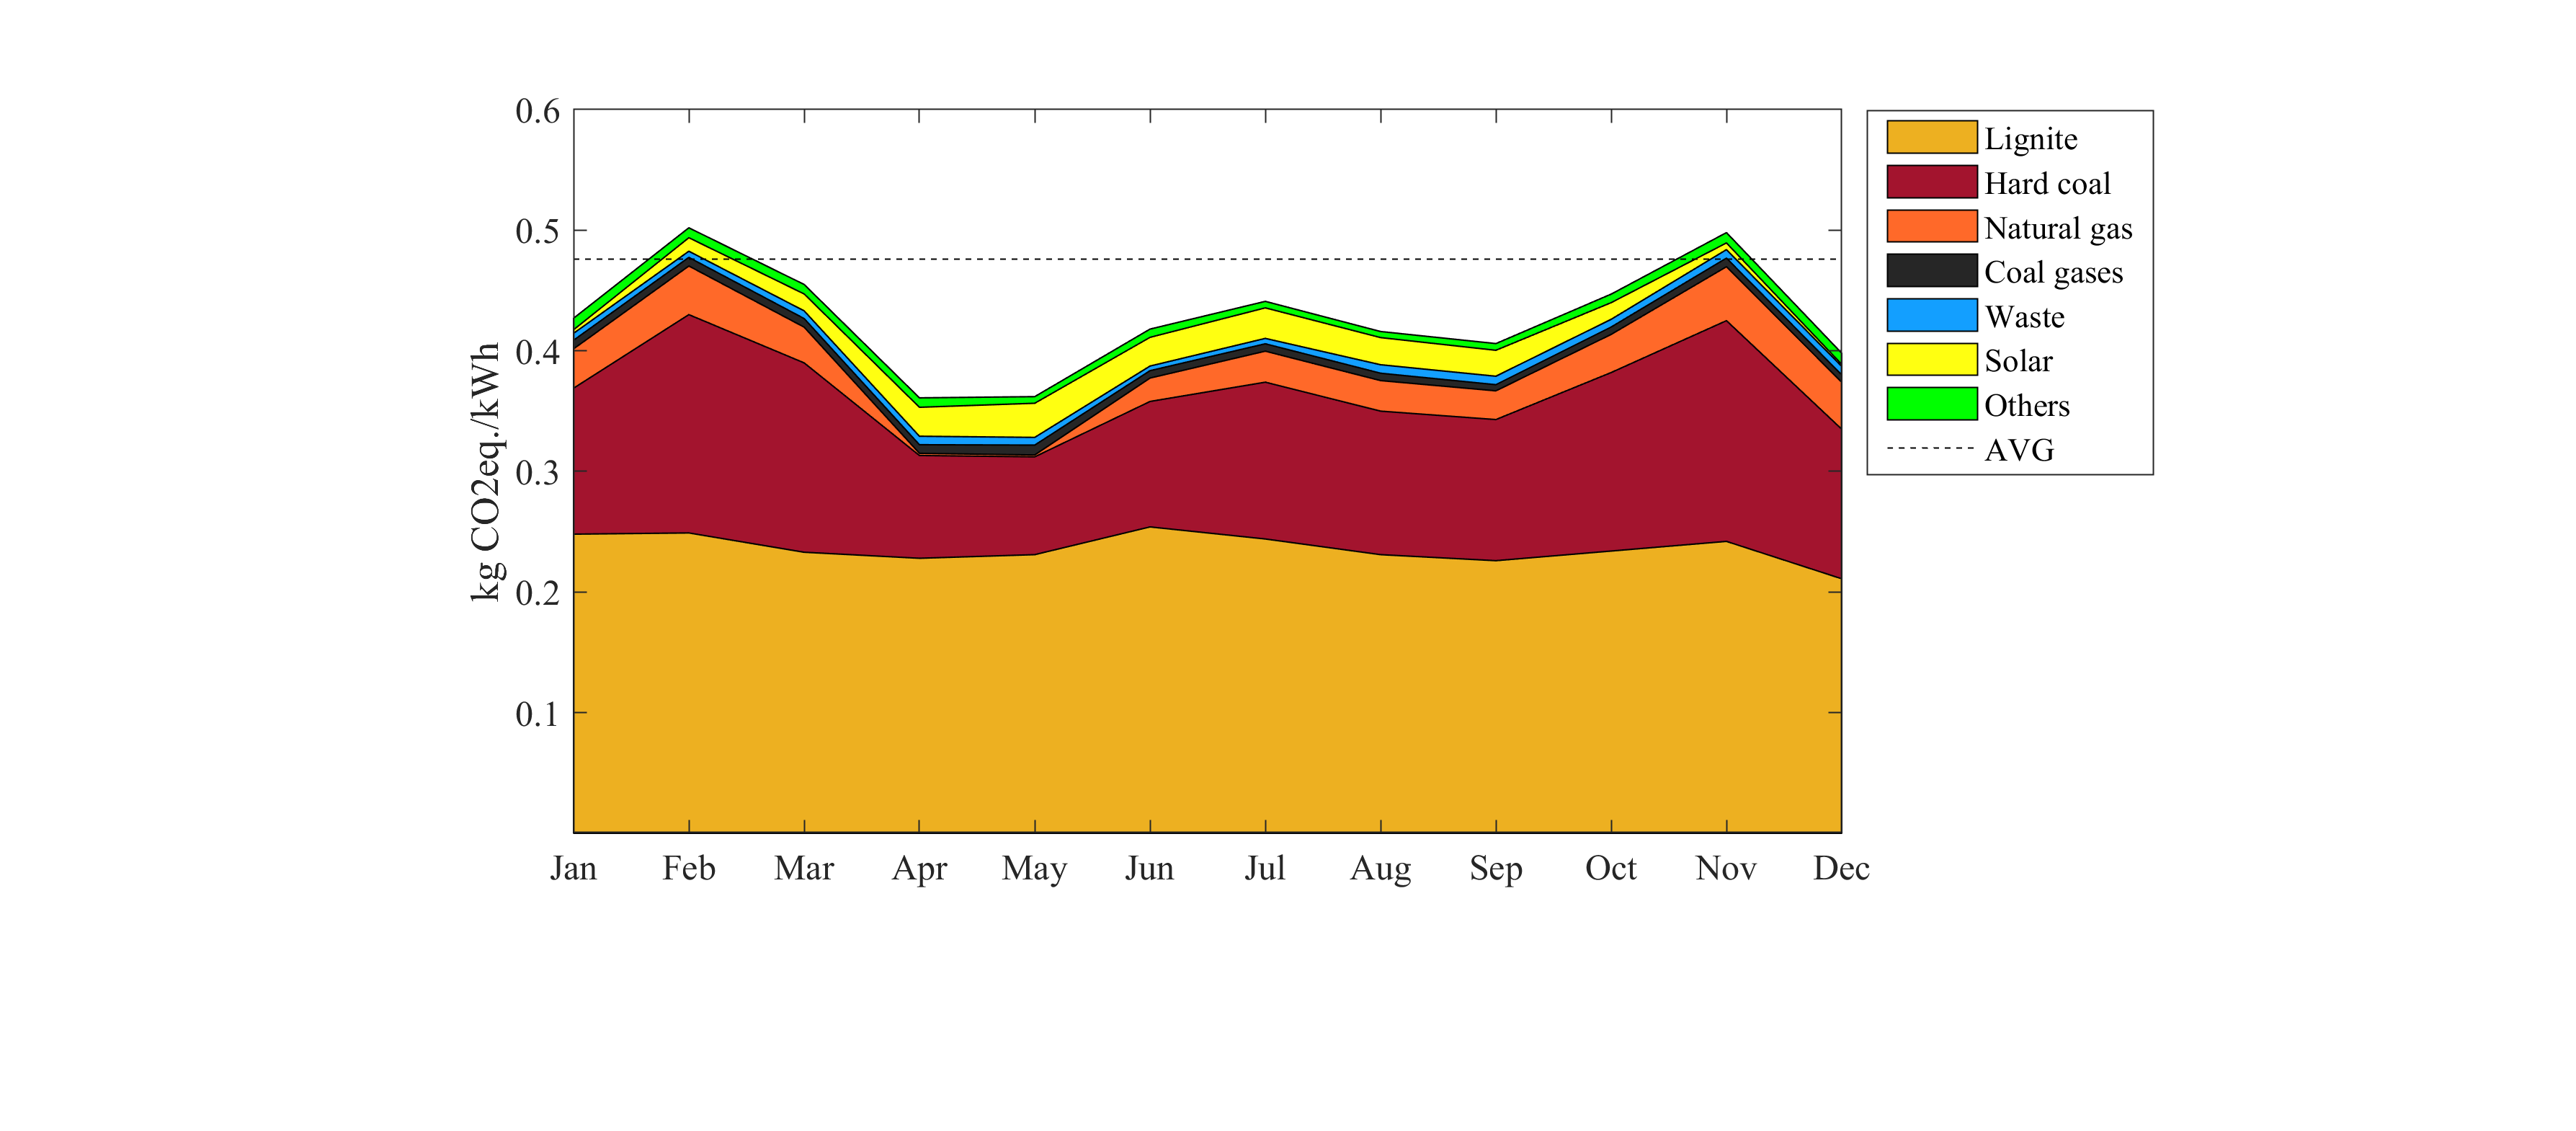
\includegraphics[width=1.2\textwidth]{ChapterLCA/Images/GWP_plots/Germany_GWP.png}
	\vspace*{-20mm}
	\caption{Monthly peak hours GWP compared with average through the year (dotted line) in Germany.}
	\label{GWP_DE}
\end{figure}
	
\begin{figure}[]
	\centering
		\hspace*{-1.6cm}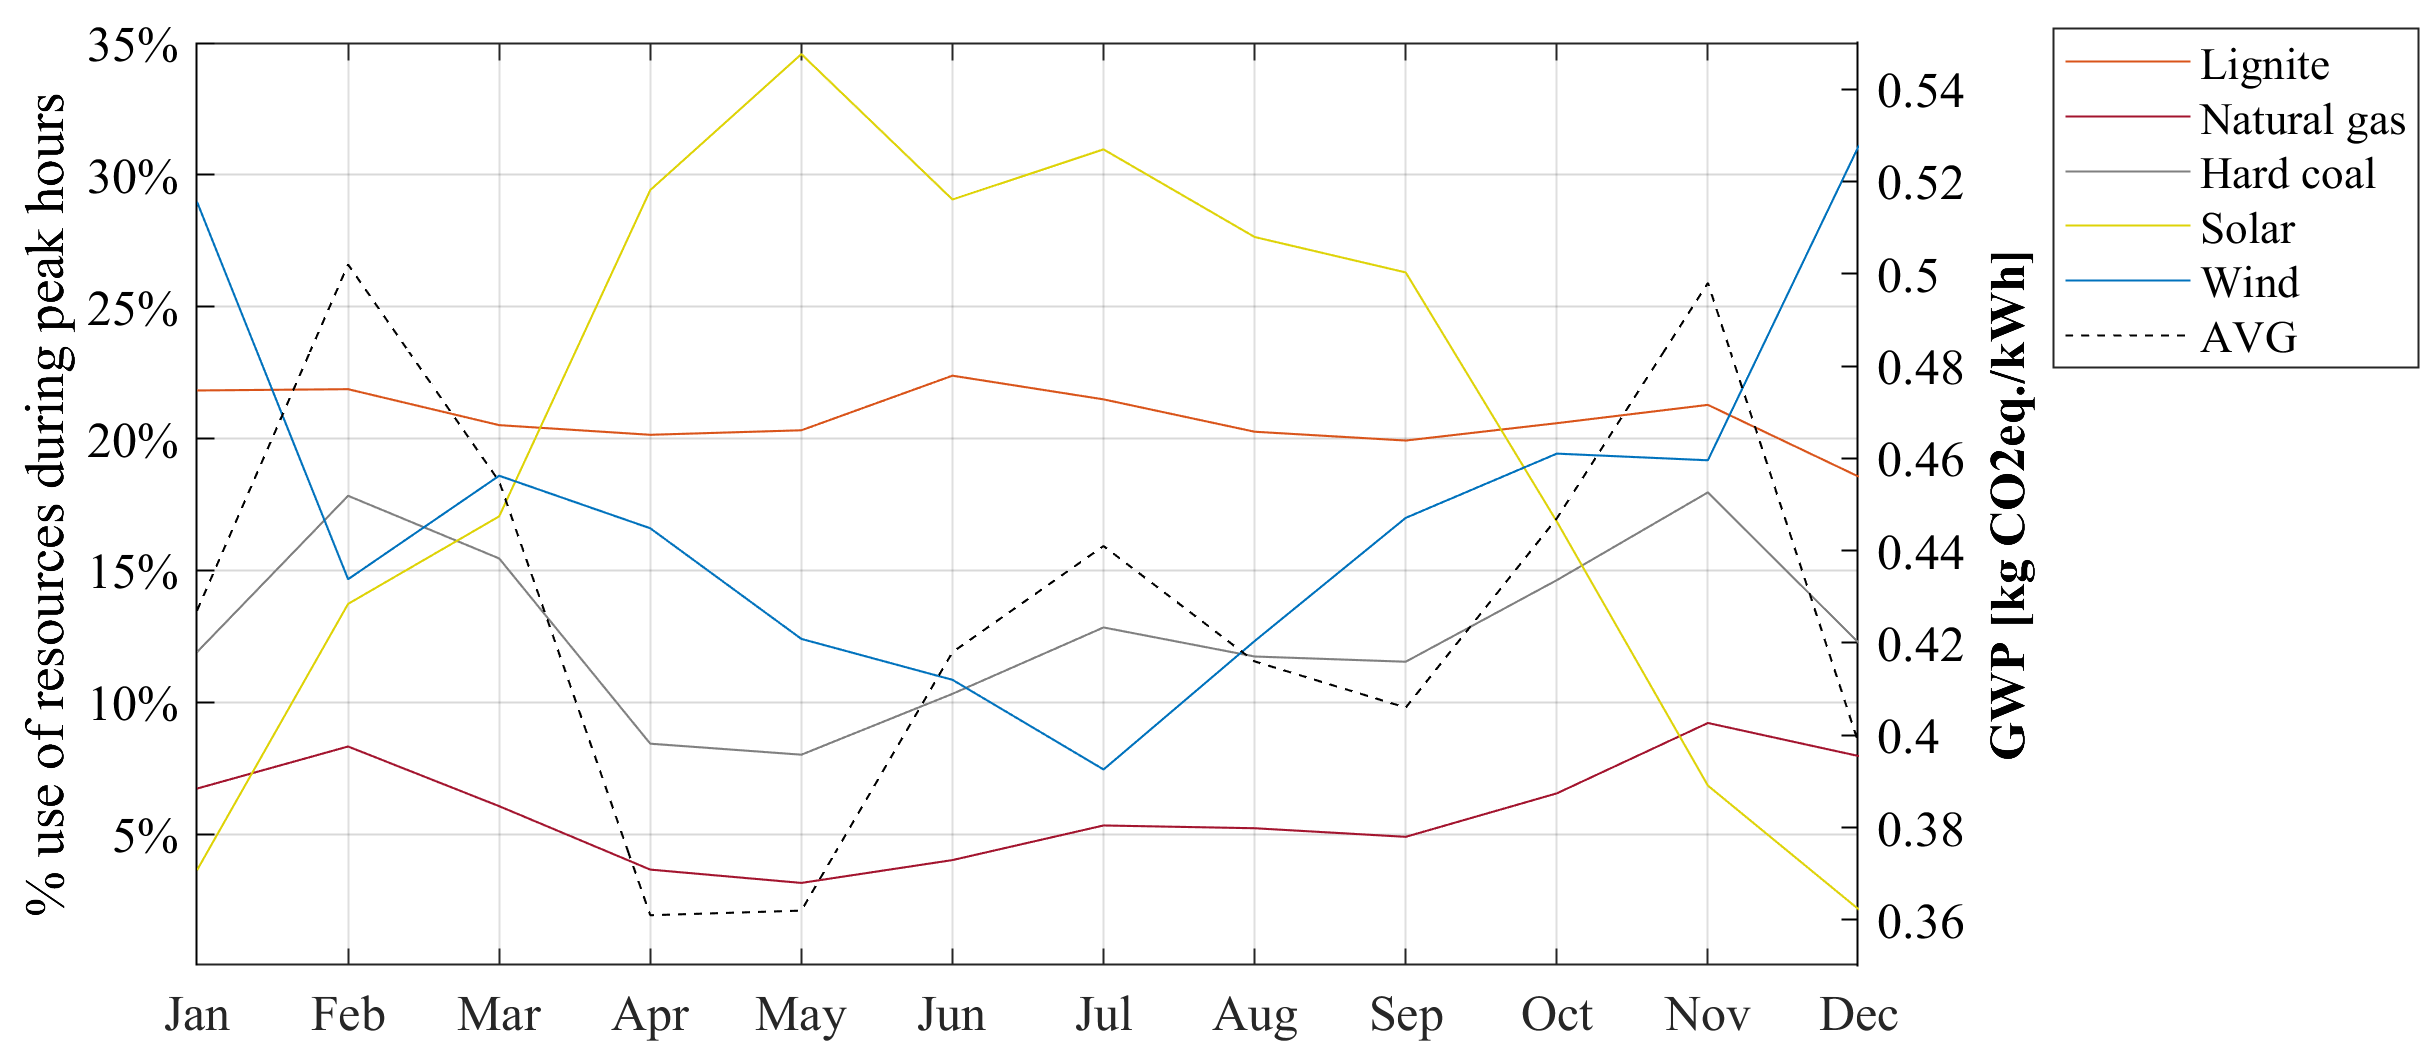
\includegraphics[width=1.2\textwidth]{ChapterLCA/Images/GWP_plots/COMP_GWP_DE.png}
	\vspace*{-20mm}
	\caption{Percentage use of resources throughout the year compared with monthly GWP in Germany, both related to peak hours.}
	\label{COMP_GE}
\end{figure}

\newpage
According to the LCIA, the GWP during peak hours was higher than the average only in  February {(+5.2\%)} and November {(+4.52\%)} (Figure \ref{GWP_DE}). This was due to the highest percentages of the use of hard coal {(+29.15\% in average)} and natural gas {(+26.1\% in average)} during the entire year, and also the higher use of lignite in comparison with the other months. From Figure \ref{GWP_DE}, April and May were the months with the lowest GWP {($-$23.95\%)}, because of the lower use of fossil fuels compared to the average. This strategy was applicable considering that both months had peaks of demand much lower than the average, {with the power requested during peak hours being around 5.45\% lower compared to the other months}. This means that the base power from nuclear power plants (which is almost constant throughout the year) had a more important role than during the months in which the production was higher and so fewer fossil fuels had to be used. It is interesting to look at solar and wind power trends: electricity production from solar power was clearly higher during the summer months, while the wind production had its maximum in the winter months (Figure \ref{GWP_DE}). These two facts lead the peak hour GWP to be lower than the average  for 10 out of 12 months. February and November, the two exceptions, saw a larger use of fossil fuels compared to the {other}%was "near", confirm. %authors: confirmed 
~months. 

%%%%%%%%%%%%%%%%%%%%%%%%% NL %%%%%%%%%%%%%%%%%%%%%%%%%%%%%%%

\subsubsection{The Netherlands}

In the Netherlands, the use of natural gas for electricity production represented  67.85\% of the total. It was the most important resource affecting the GWP value. Nuclear power helped to cover a small percentage of the base load {(6.61\%)}, while the lack of hydropower capacity influenced the electricity generation strategy.  The overall production percentages are presented in Table \ref{RES_NL}.  The total electricity produced during the year in the country was equal to 224.8 TWh.

 \begin{table}[]
\centering
\caption{Percentage of resources used during peak and off-peak hours in the Netherlands \cite{Entso-eProduction}.}
\label{RES_NL}
\begin{tabular}{ccccc}
\toprule
\textbf{Natural Gas} & \textbf{Wind} & \textbf{Nuclear} & \textbf{Solar}  & \textbf{Biomass}  \\ \hline
      67.85\%       & 19.48\%        & 6.61\%           & 5.48\%           & 0.58\%         \\ \bottomrule
\end{tabular}
\end{table}

 Through the analysis related to the ENTSO-E data \cite{Entso-eProduction}, the yearly average value was 0.287 kg CO\textsubscript2-eq/kWh. In the study performed by Moro et al. \cite{Moro2017}, the average outcome for the GWP was 0.558 kg CO\textsubscript2-eq/kWh. The reason behind this difference lies in the fact that hard coal electricity production in the Netherlands was not mentioned by the ENTSO-E TP for 2018. However, hard coal has still a considerable percentage in the energy mix, as is notable in Table \ref{table:capacity}. This lack of data reduces the accuracy of the GWP results, but not the effect of the other resources on peak hours. As is notable from Figure \ref{GWP_NL}, hard coal is not specified.  
 
 As can be seen in Figure \ref{COMP_NL}, the GWP line follows the natural gas use curve. The valley formed by the dotted line from March to June is linked to a similar one drawn by the natural gas curve. From April until July, the amount of electricity produced through solar power plants during peak hours was higher than the yearly average, resulting in an increase of {+39.7\% on average}, affecting positively the GWP. The lowest values for wind production corresponded to the highest values of the GWP (Figure \ref{GWP_NL}), {as in February, when the production from wind power was 49.94\% lower than the yearly average}. The changes in the use of  resources through the year were limited, and this is why there were no major changes in monthly GWPs. {The Netherlands was the country with the lowest observed fluctuations in terms of GWP, being in the range between 0.256 and 0.303 kg CO\textsubscript2-eq/kWh (respectively $-$10.9\% and +5.6\% in comparison with the yearly average value of 0.287 kg CO\textsubscript2-eq/kWh). As already observed in the case of Germany, solar and wind power had opposite concavities. When the availability of solar and wind power during peak hours was higher than the average, lower values of GWP were obtained.} 
 

\begin{figure}[]
	\centering
	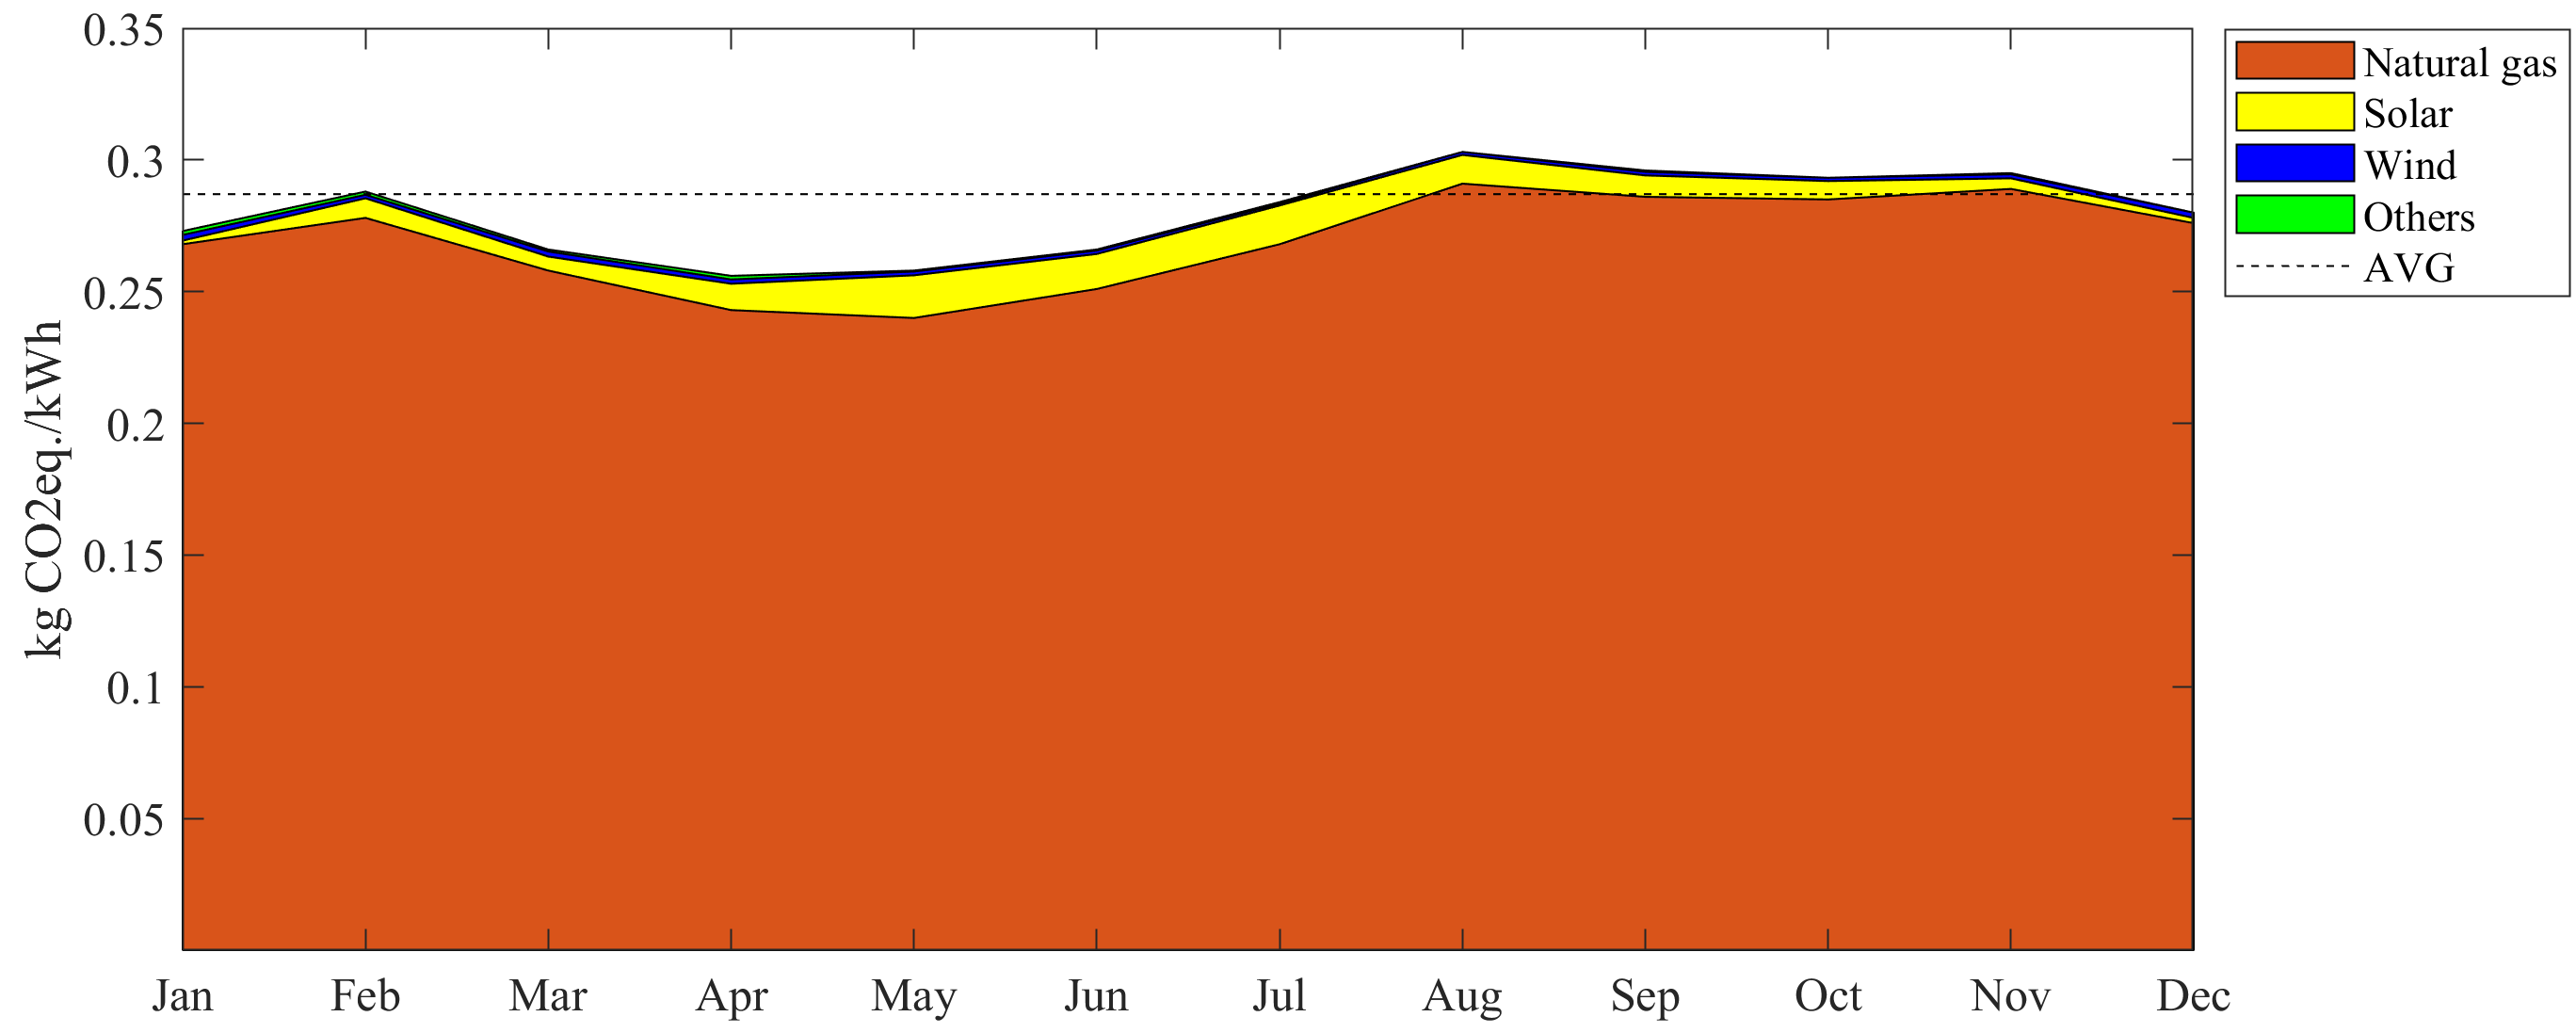
\includegraphics[width=1\textwidth]{ChapterLCA/Images/GWP_plots/Netherlands_GWP.png}
	\vspace*{-17mm}
	\caption{Monthly peak hours GWP compared with the annual average (dotted line) in the Netherlands.}
	\label{GWP_NL}
\end{figure}
	
\begin{figure}[]
	\centering
	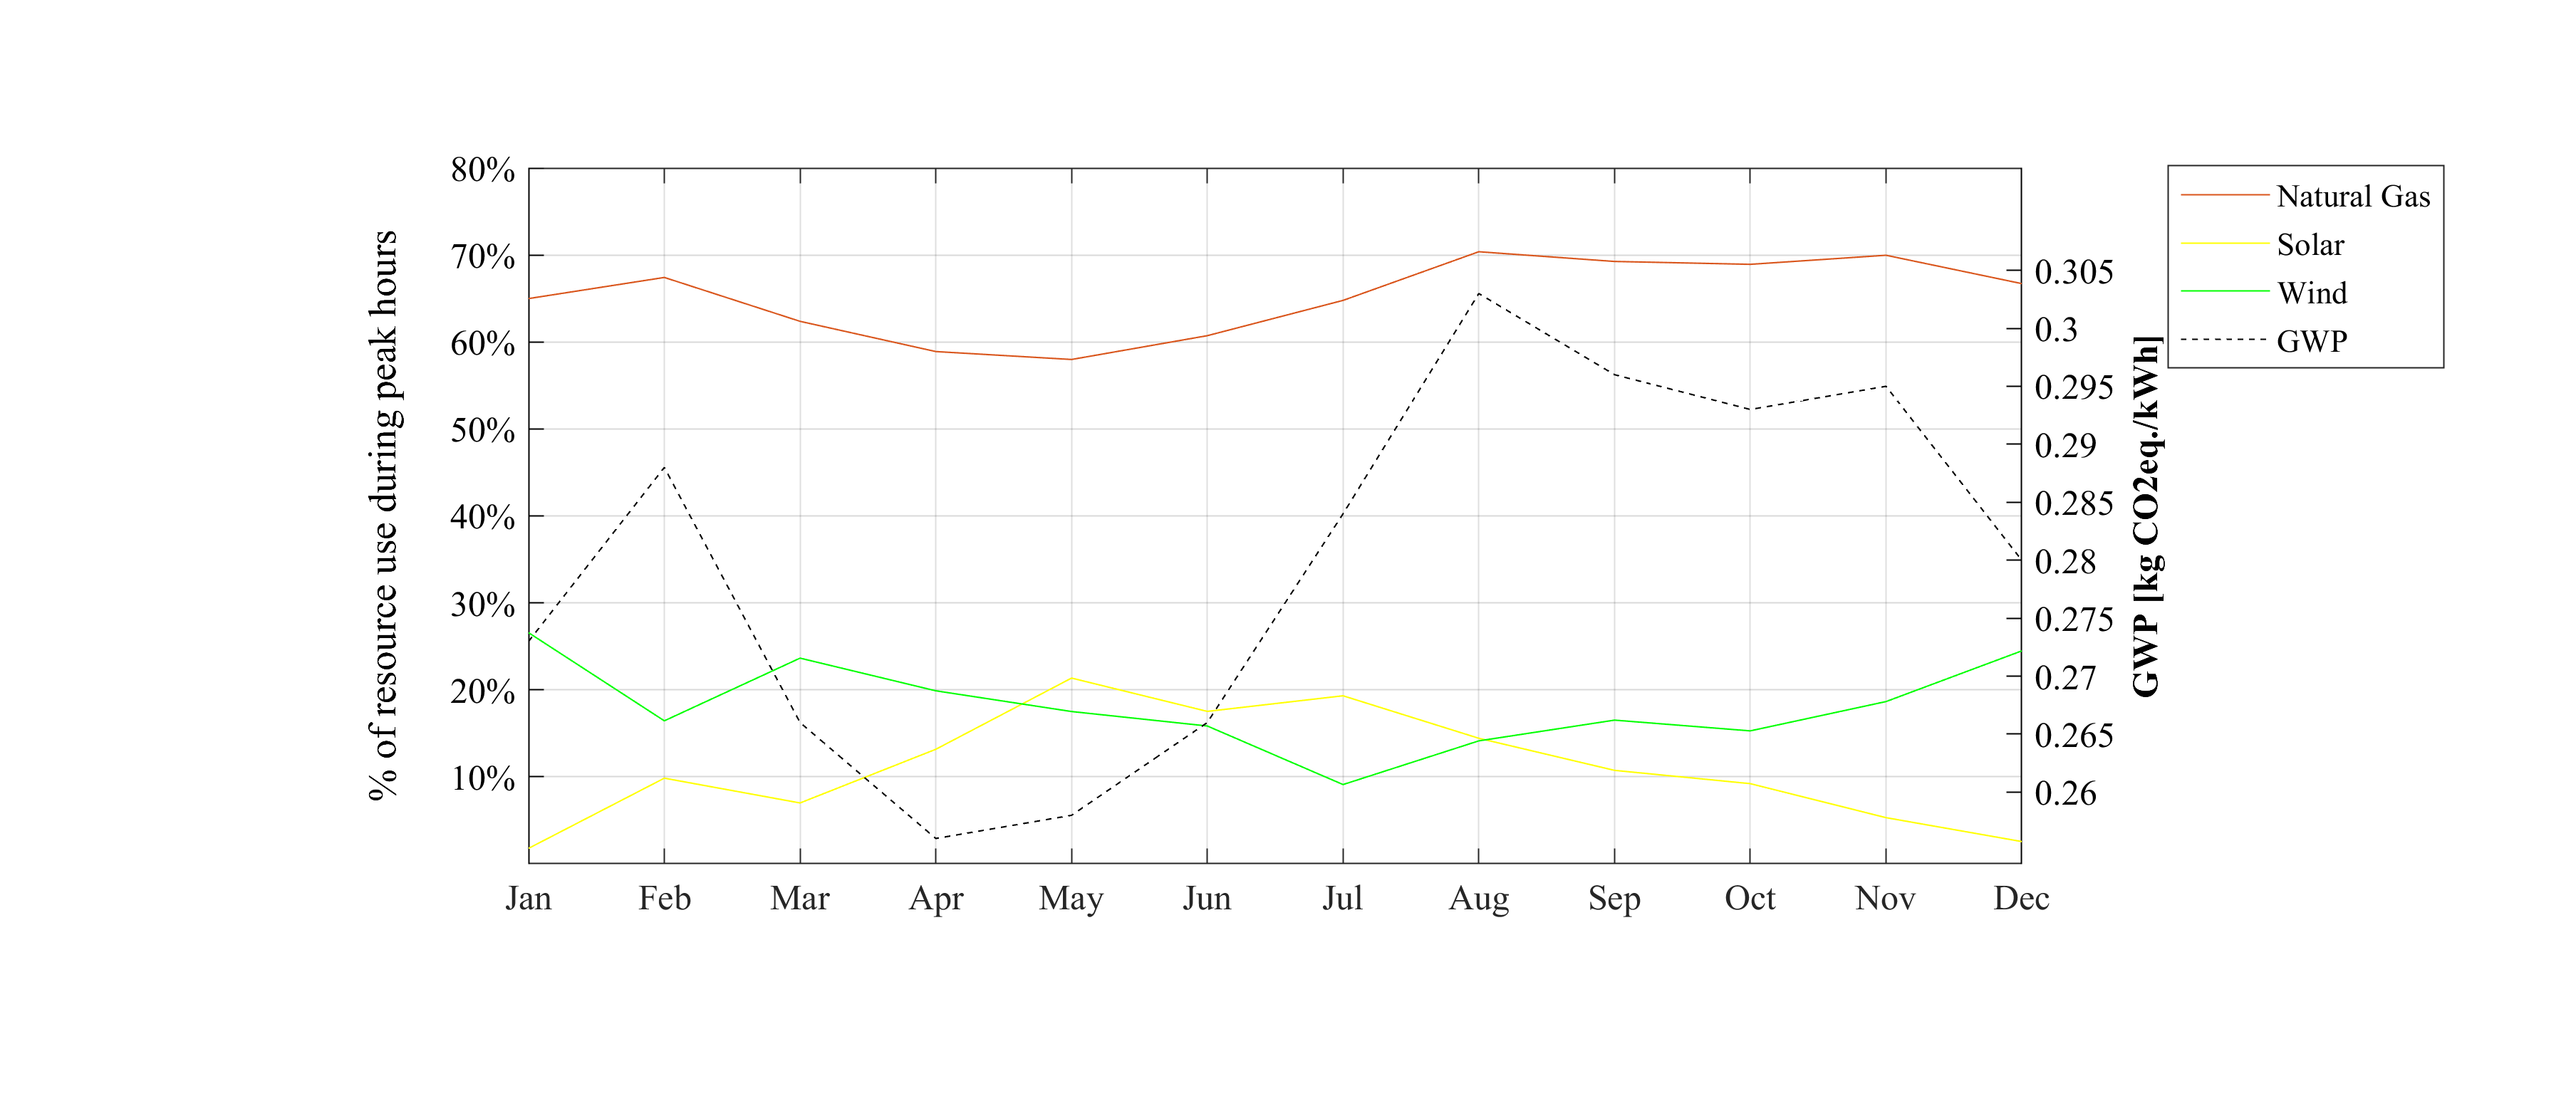
\includegraphics[width=0.9\textwidth]{ChapterLCA/Images/GWP_plots/Comp_GWP_NL.png}
		\vspace*{-8mm}
	\caption{Percentage use of resources throughout the year compared with monthly GWP in the Netherlands, both related to peak hours.}
	
	\label{COMP_NL}
\end{figure}


 
%%%%%%%%%%%%%%%%%%%%%%%%% NO %%%%%%%%%%%%%%%%%%%%%%%%%%%%%%%

\subsubsection{Norway}
As mentioned in Table \ref{RES_NO}, Norway bases its electricity needs on hydropower. The high percentage of water reservoirs and pumped hydro storage {(87.93\%)} allows the Nordic country to manage the generation in a flexible manner.  Thanks to this, the GWP value related to the produced electricity was much lower compared to the other studied countries, {being around an order of magnitude less}. Although it is beneficial for the flexibility of the generation, Norway is a good example of a country in which pumped hydro is not actually valuable because of the high presence of naturally charged reservoirs. The pumped storage technology was just a small percentage compared with the conventional hydropower (see Table \ref{table:capacity}). Its use is historically based in the months of June and July \cite{Kougias2017PumpedHorse}. Regarding the case study of 2018, a greater use in May was also observed. PHS%Define if appropriate #authors: we have defined it previously, and so the abbreviation can be used here. 
~is used to store the electricity that comes from conventional thermal power plants, leading to higher GWP values during those months, as presented in Figure \ref{GWP_NO}. The total electricity produced during the year in the country was equal to 146.8 TWh.

 \begin{table}[]
\centering
\caption{Percentage of resources used during peak and off-peak hours in Norway \cite{Entso-eProduction}.}
\label{RES_NO} 
\begin{tabular}{ccccc}
\toprule
\textbf{Hydro Reservoir} & \textbf{Hydro Run-of-River} & \textbf{Wind Onshore} &  \textbf{Natural Gas}   & \textbf{Others}  \\ \hline
87.93\%                & 6.87\%  & 2.32\% &2.10\%                     &                  0.77\%                         \\ \bottomrule
\end{tabular}
\end{table}


\begin{figure}[]
	\centering
	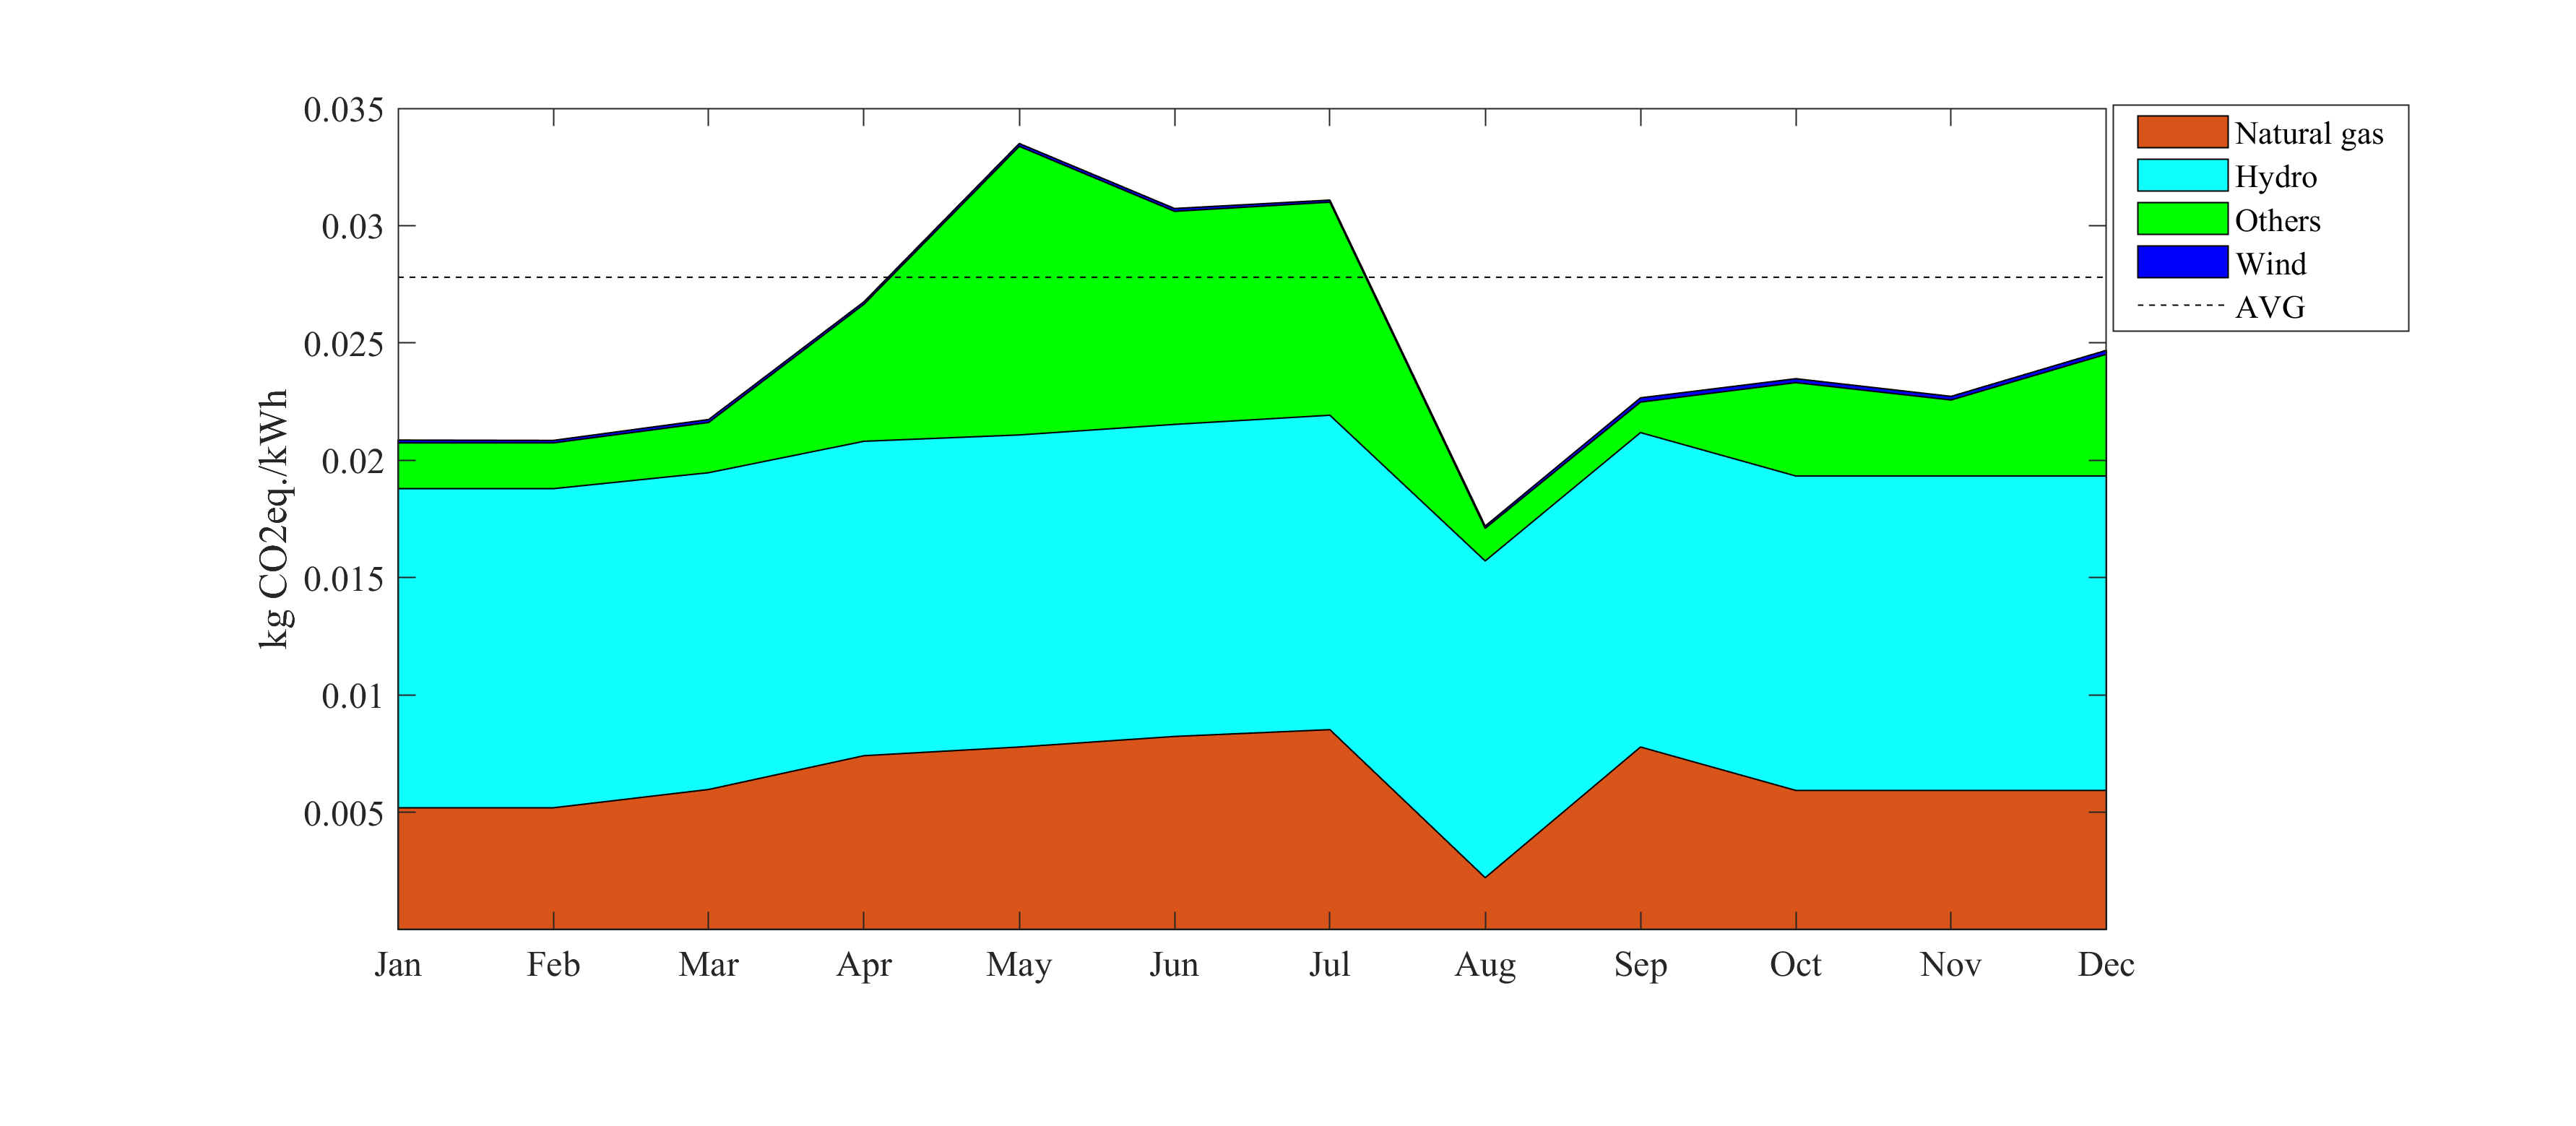
\includegraphics[width=0.9\textwidth]{ChapterLCA/Images/GWP_plots/Norway_GWP.png}
	\vspace*{-8mm}
	\caption{Monthly peak hours GWP compared with average through the year (dotted line) in Norway.}
	\label{GWP_NO}
\end{figure}
\vspace*{-5mm}
\begin{figure}[]
	\centering
	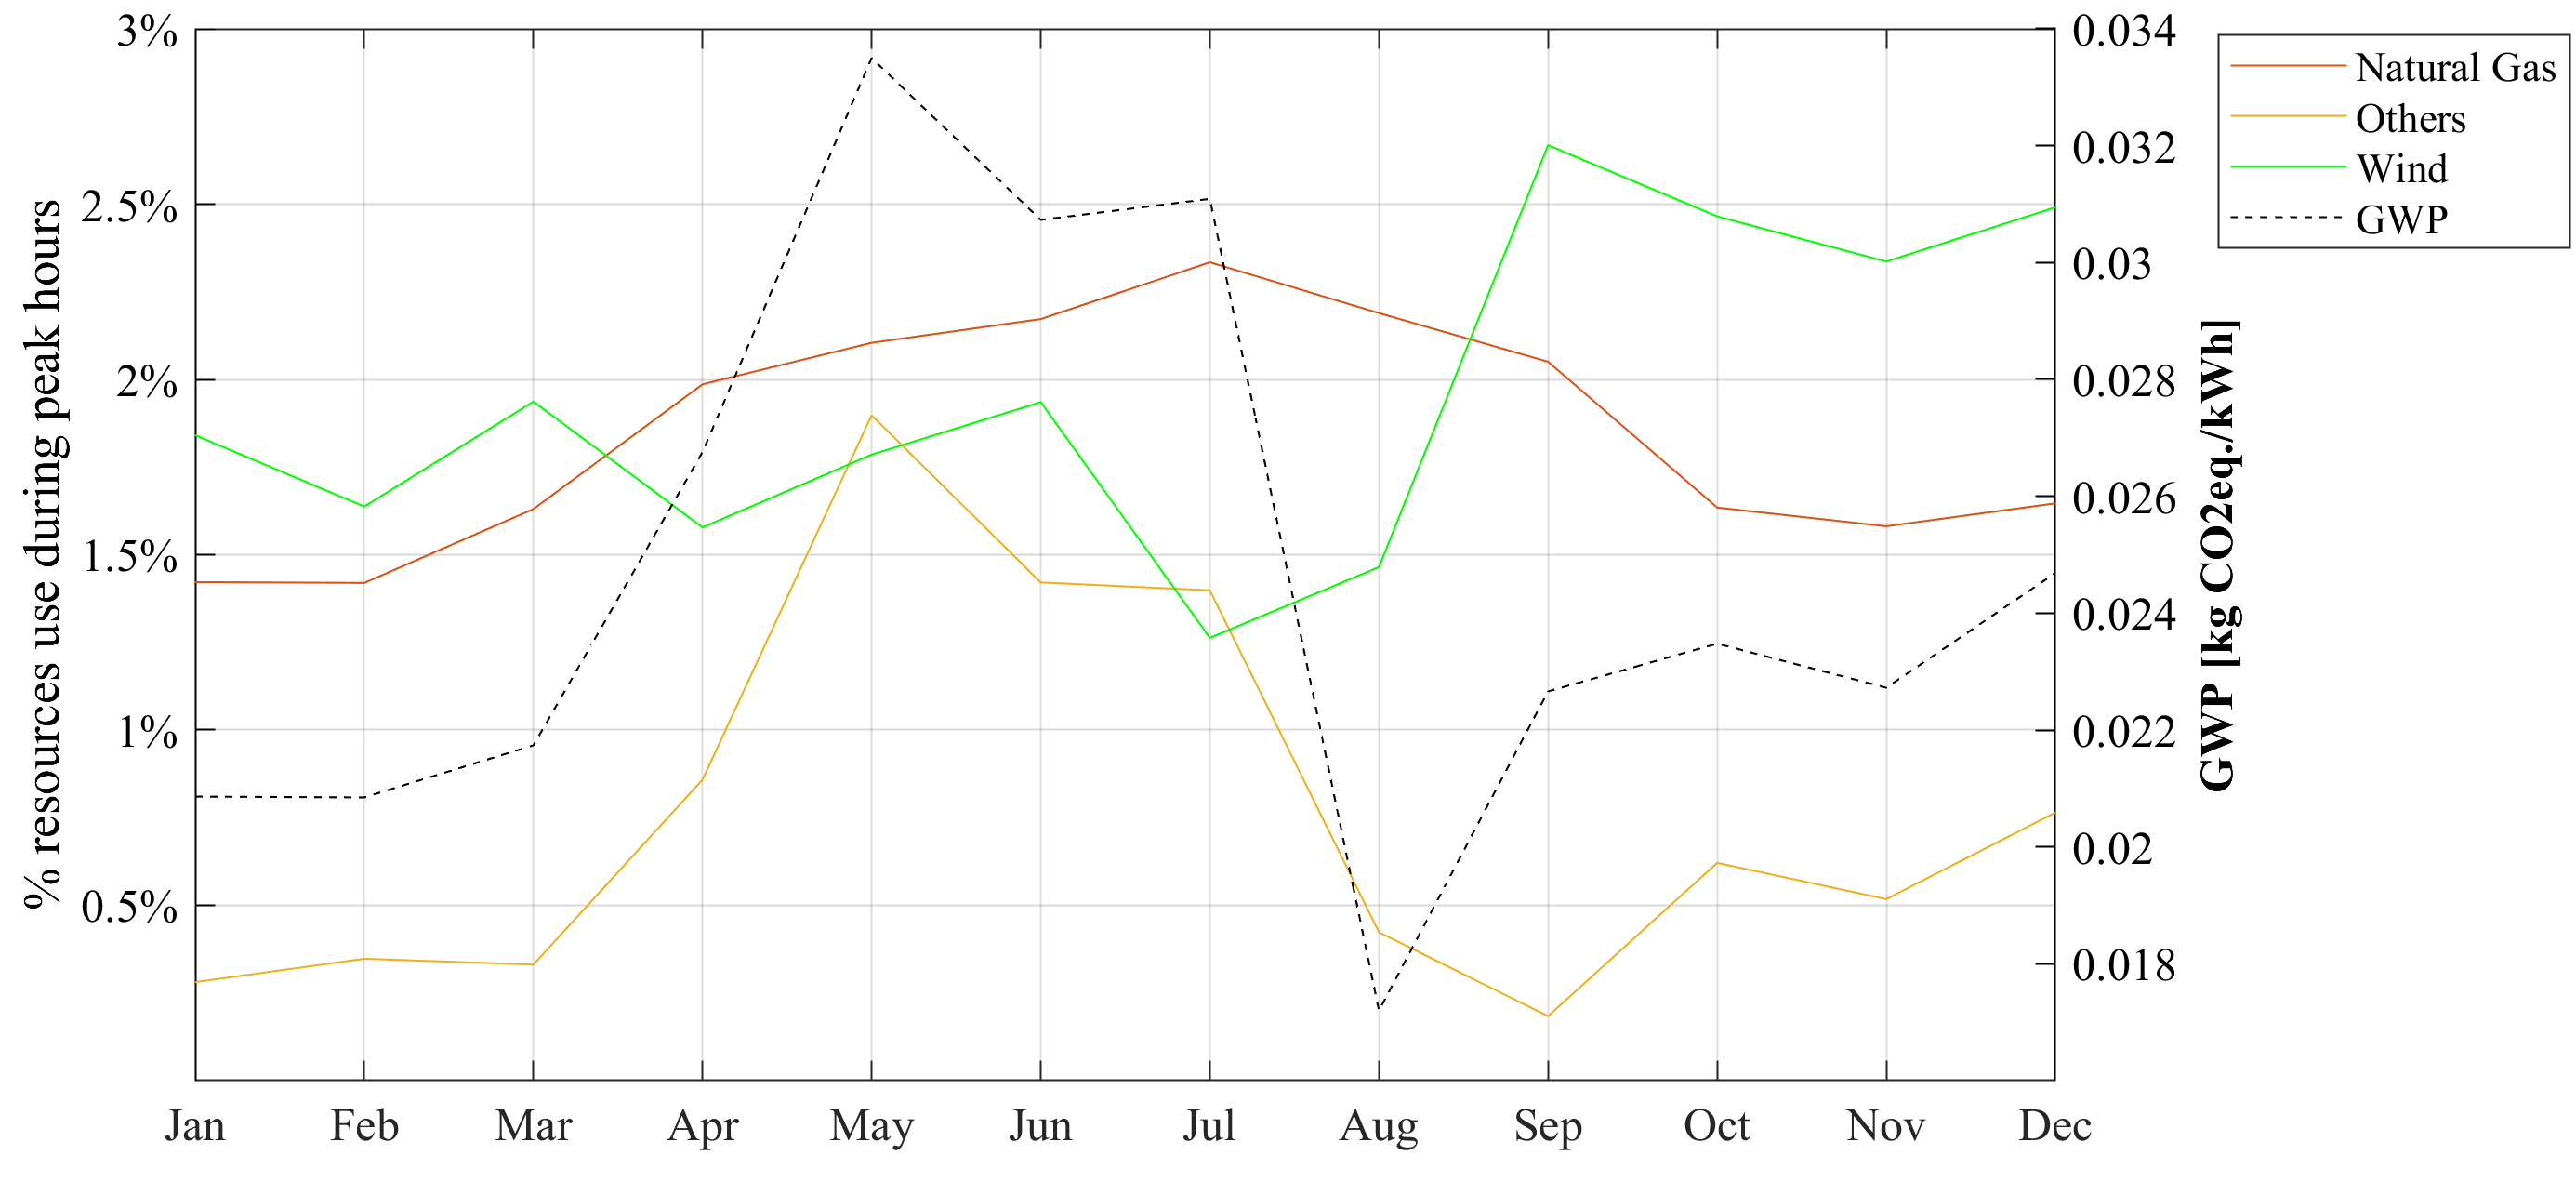
\includegraphics[width=0.95\textwidth]{ChapterLCA/Images/GWP_plots/Comp_GWP_NO.png}
    \vspace*{-8mm}
	\caption{Percentage use of resources throughout the year compared with monthly GWP in Norway, both related to peak hours.}
	\label{COMP_NO}
\end{figure}

 According to Figure \ref{GWP_NO}, what was not produced with reservoirs and pumped storage was mainly  made by natural gas, wind, and waste power plants. This is why the GWP line follows the ``Others'' resources use curve for the majority of the year 2018. Whenever there was more production from waste {(+42.5\% in average)} and natural gas {(+18.9\% on average)}, the GWP was higher than the average (Figure \ref{COMP_NO}). {Curiously, the months of May, June, and July were also the ones with the lowest power generation during peak hours.} During the month of August, the amount of power required for the nation's needs was close to the yearly average, but fewer thermal power plants were used while hydropower plants were even more exploited than usual, {leading August to be the month with the lowest GWP of the year, with a value of 0.0172 kg CO\textsubscript2-eq/kWh. %Should this be "$_{2\mathrm{eq.}}$"? Authors: We have changed it according to the standards for all the cases in the text.
 Nevertheless, the monthly changes in the use of all the resources was always lower than 2\% and this is why also the GWP did not differ substantially. 

%%%%%%%%%%%%%%%%%%%%%%%%% ES %%%%%%%%%%%%%%%%%%%%%%%%%%%%%%%
\subsubsection{Spain}

Spain has several different resources with a great share in the electricity production, like Germany.
 Natural gas and hard coal were the fossil fuels used at higher rates, with percentages of 20.91\% and 13.29\% respectively. Nuclear power plants accounted for 22.46\% of the total yearly electricity production, and  wind onshore power represented a consistent share (20.21\%).  Solar production was also present  during night hours because of some concentrated solar power plants with molten salts. Table \ref{RES_ES} shows the resources used during the year in descending order. The total electricity produced during the year in the country was equal to 242.7 TWh.

 \begin{table}[]
\centering
\caption{Percentage of resources used during peak and off-peak hours in Spain \cite{Entso-eProduction}.}
\label{RES_ES}
\resizebox{\textwidth}{!}{%
\begin{tabular}{ccccccccc}
\hline
 \textbf{Nuclear} & \textbf{Natural Gas} & \textbf{Wind} & \textbf{Hard Coal} & \textbf{Hydro}  & \textbf{Solar} &\textbf{Lignite}  &\textbf{Biomass} & \textbf{Others*} \\ \hline
22.46\%  & 20.91\%       & 20.21\%                   & 13.29\%            & 13.22\%                  & 4.69\%         & 1.28\%   & 1.25\%     & 2.32\%             \\ \hline
\end{tabular}%
}
%\begin{tablenotes}
%   \vspace*{3mm}
%      \small
%      \item *Others includes: Fossil Oil, Other renewables and Waste
%    \end{tablenotes}
\begin{tabular}{ccc}
\multicolumn{1}{c}{\footnotesize*Others includes: fossil oil, other renewables, and waste.}
\end{tabular}

\end{table}



\begin{figure}[]
	\centering
	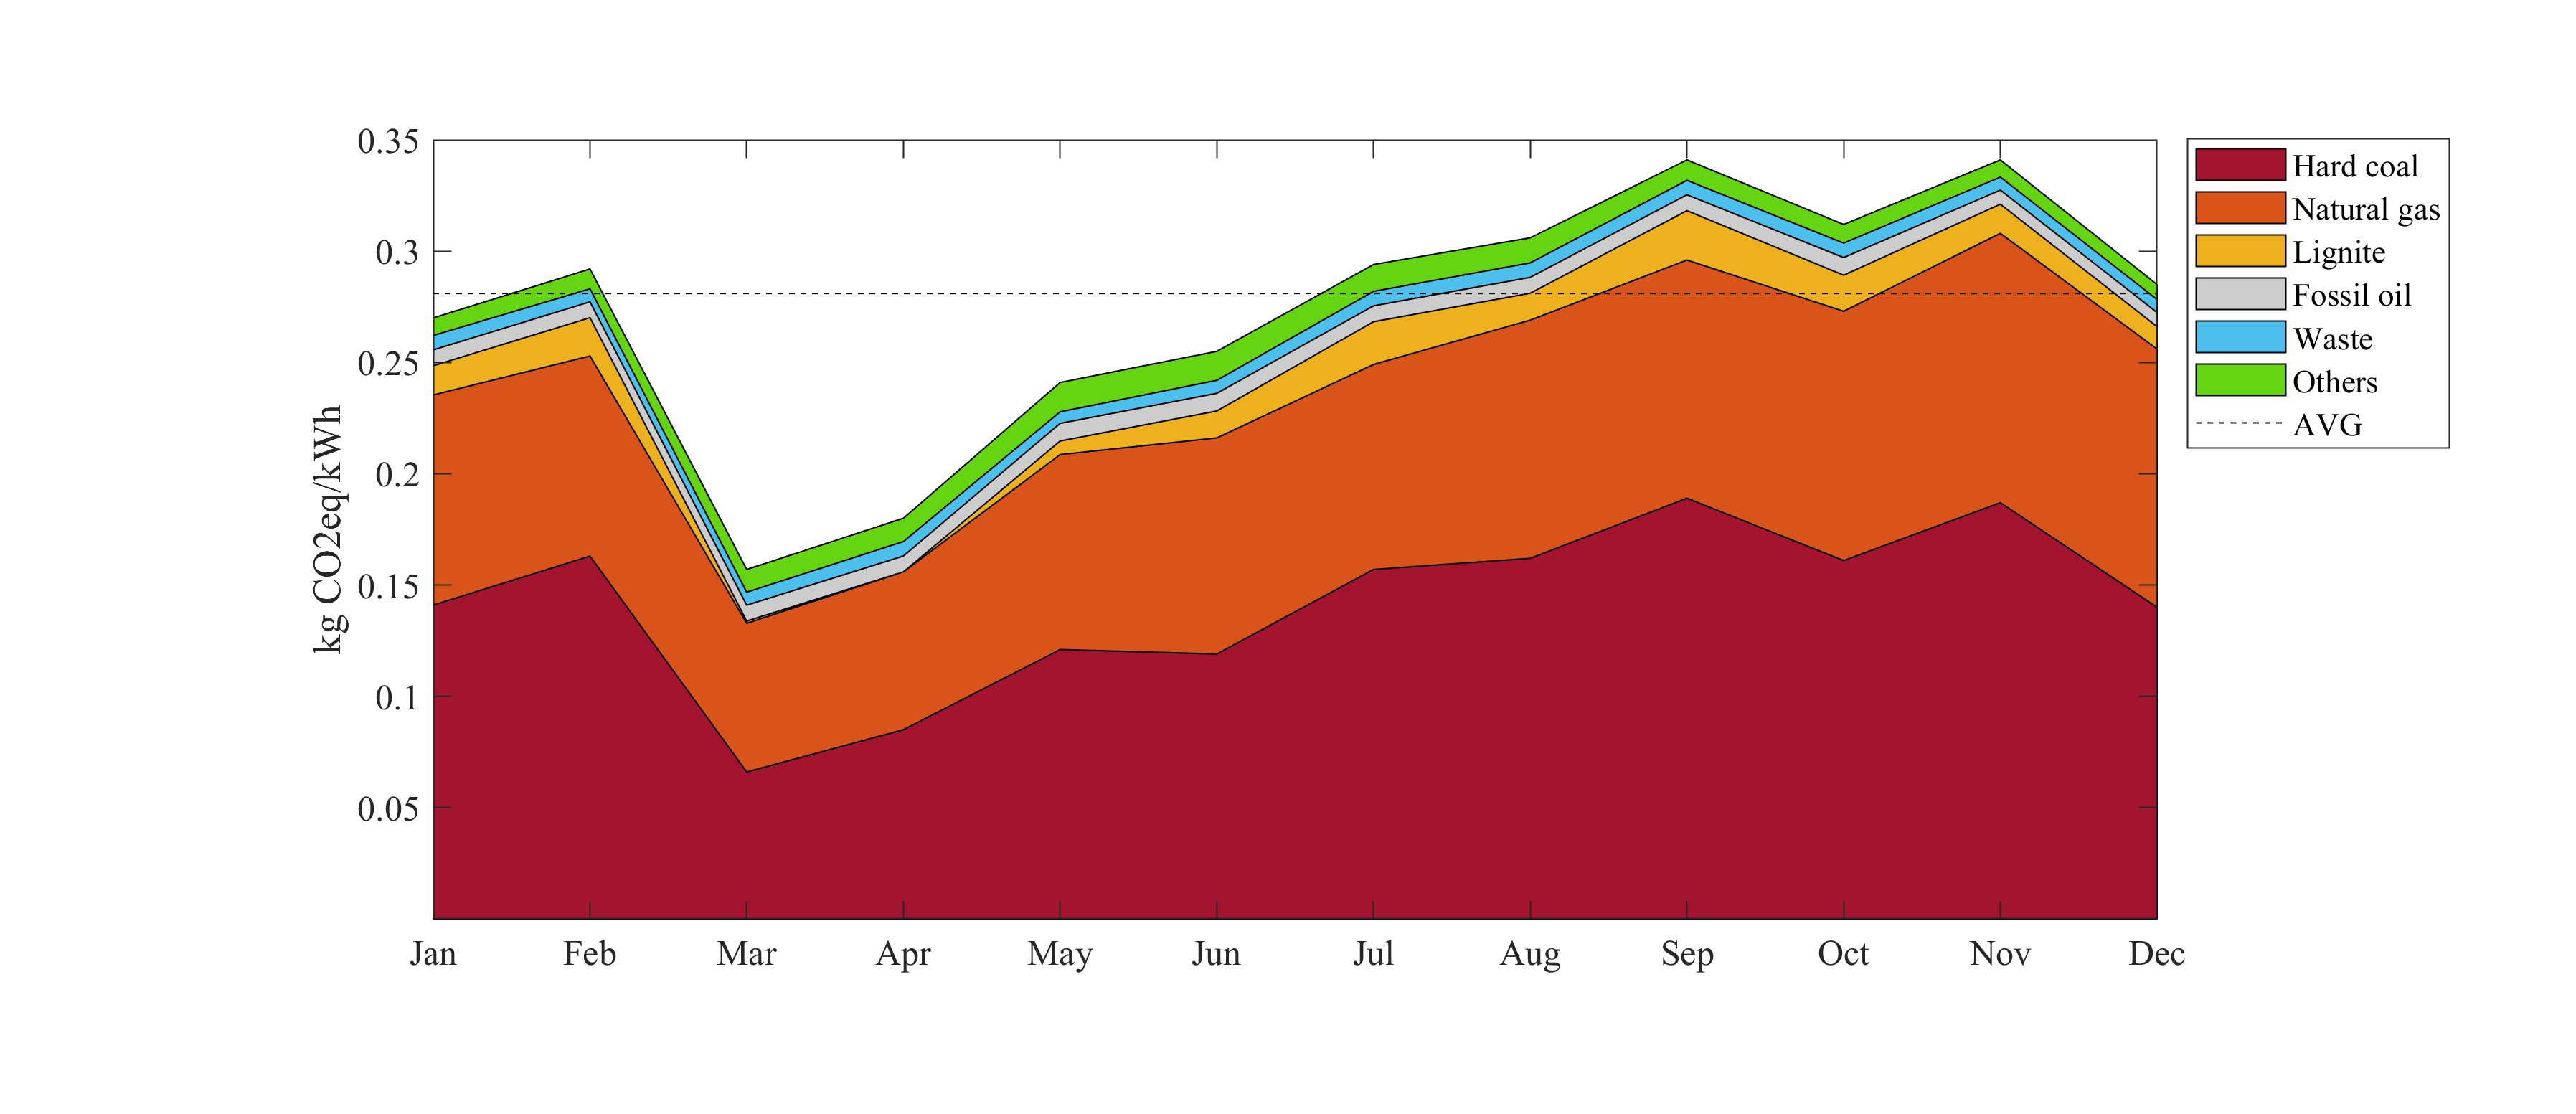
\includegraphics[width=0.95\textwidth]{ChapterLCA/Images/GWP_plots/Spain_GWP.png}
	\vspace*{-7mm}
	\caption{Monthly peak hours GWP compared with average through the year (dotted line) in Spain.}
	\label{GWP_ES}
\end{figure}
	\vspace*{-7mm}
\begin{figure}[]
	\centering
	\hspace*{0.3cm}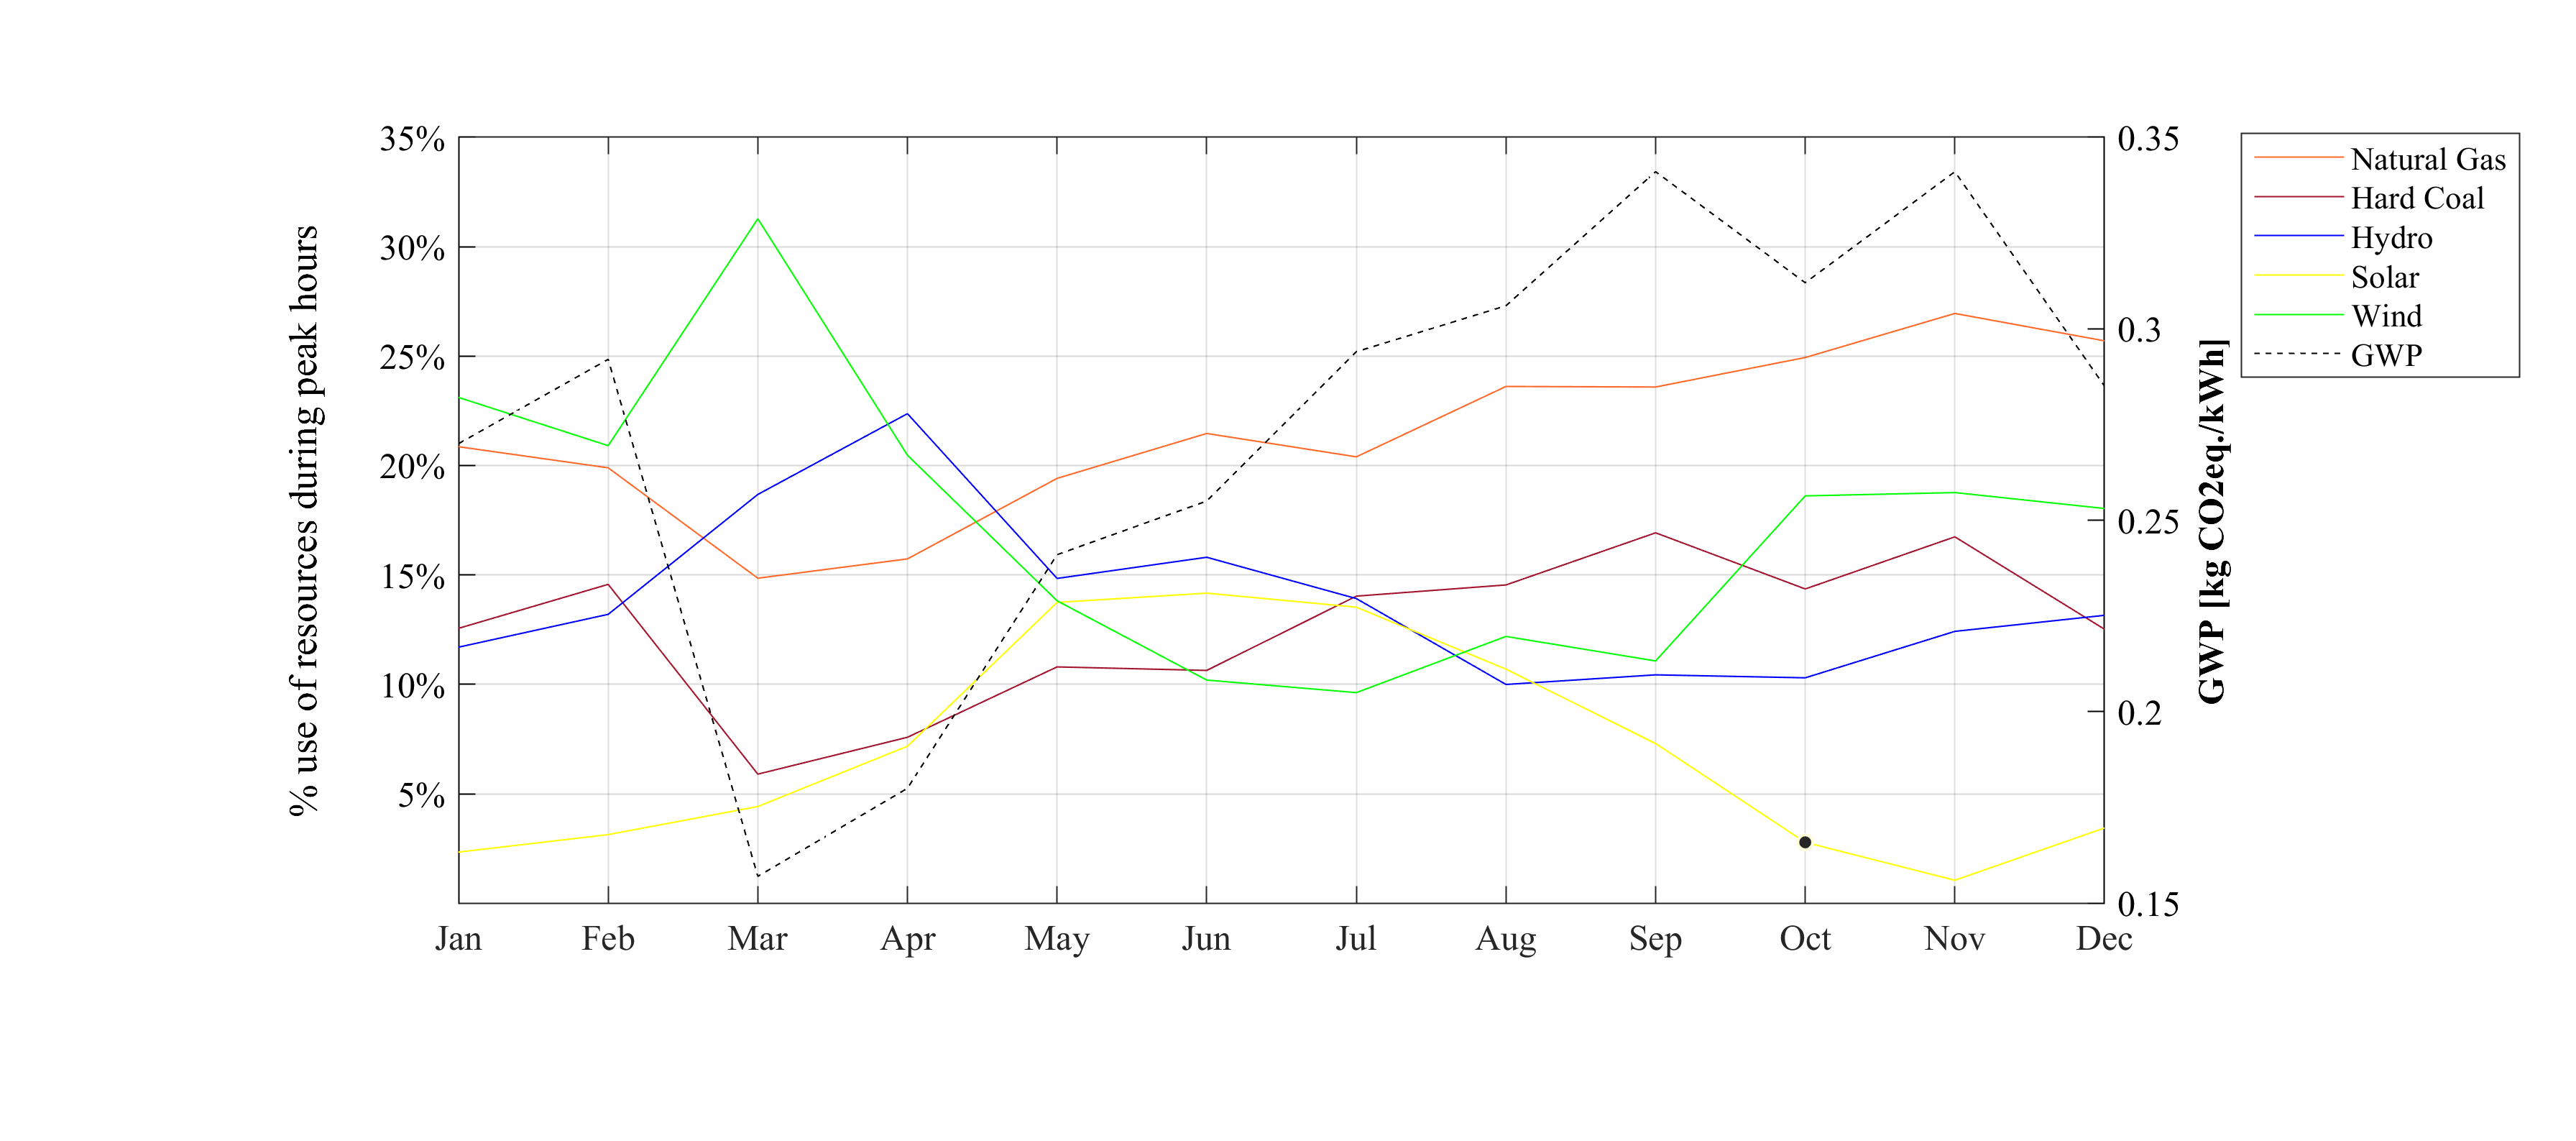
\includegraphics[width=0.95\textwidth]{ChapterLCA/Images/GWP_plots/Comp_GWP_ES.png}
	\vspace*{-10mm}
	\caption{Percentage use of resources throughout the year compared with monthly GWP in Spain (both related to peak hours).}
	\label{COMP_ES}
\end{figure}

The dependence on  fossil fuels resulted in a high GWP in Spain. Figure \ref{GWP_ES} demonstrates that natural gas and hard coal were the main drivers of a high GWP, and the less they were used, the lower the indicator was. Figure \ref{COMP_ES} shows that during the month of March there was a minimum of the GWP value {(0.157 kg CO\textsubscript2-eq/kWh}, due to a high production of wind power which reached 30\% of the share of production and at the same time an increase in the use of hydro storage and solar power plants. The two maximum GWP points recorded in September and November, {both  0.341 kg CO\textsubscript2-eq/kWh, were due to a decrease in solar electricity production and a consequential increase of fossil fuels to meet the demand needs (Figure~\ref{COMP_ES}). {Spain was the analyzed country with the highest fluctuations among the different months of the year. March had the lowest GWP, being 44.2\% lower than the average value. On the contrary, September and November had the greatest GWP values, specifically 21.3\% higher than the annual average value of 0.281~kg CO\textsubscript2-eq/kWh.


%%%%%%%%%%%%%%%%%%%%%%%%%%%%%%%%%%%%%%%%%%%%%
\section{Discussion} \label{Discussion}

The effects of temporal variability on GWP values confirmed their importance in this study. Impact indicators can differ substantially depending on the amount of power produced, the season, and the resources used throughout the year. The expectation to obtain higher GWP values during peak hours in comparison with the annual average value was not completely confirmed here. In fact, many factors can cause variations in the GWP during different periods, such as the marginal technology used in peak hours and the baseline technology, which can make a difference in the overall GWP value. {For this reason, it is important to consider not only economic savings but also environmental aspects when defining DR and flexibility strategies.}

%Generally, a country which has a constant base production (e.g. from nuclear), during periods in which the demand is lower than the average needs less power and consequently less fossil fuel to cover the demand, leading to lower GWP values. 

%Beyond that, the average yearly value of the GWP was calculated taking into consideration all the 8760 hours of the year 2018. However, during night times, an important low-impact resource like the sun power is not present. As a result, there are some months, especially during the summer time, in which the GWP of peak hours is lower than the average yearly value. 

During low-demand times (e.g., night hours), the power requested is lower than during peak hours, and consequently it is logical that the GWP value should be lower than the average, because less resources are used to produce the electricity. In contrast, it should be noted that the comparison was always made taking into account the functional unit equal to 1 kWh. Hence, the time slots were not compared with their  absolute production values but with relative ones, normalized to 1 kWh. For example, an hour with a power generation of 2000 MW can have a higher GWP value than a 5000 MW one, since it depends on the resources used to meet the demand. In summary, GWP is usually higher not because more electricity is produced, but because more fossil fuels are used to reach the maximum production.


%%%%%%%%%%%%%%%%%%%%% SUMMARY TABLE

% Please add the following required packages to your document preamble:
% \usepackage{multirow}
% \usepackage{graphicx}
 \begin{table}[]
\centering
\caption{Summary of results between LCA and peak-hourly life cycle assessment (PH-LCA).}
\label{summaryfindings}
\resizebox{\textwidth}{!}{%
\begin{tabular}{lllllll}
\toprule
\textbf{Approach} & \textbf{\begin{tabular}[c]{@{}l@{}}Country /\\ Indicator\end{tabular}} & \textbf{\begin{tabular}[c]{@{}l@{}}Bulgaria \\ {(}kg CO\textsubscript2-eq/kWh{)}\end{tabular}} & \textbf{\begin{tabular}[c]{@{}l@{}}Germany\\ {(}kg CO\textsubscript2-eq/kWh{)}\end{tabular}} & \textbf{\begin{tabular}[c]{@{}l@{}}The Netherlands\\ {(}kg CO\textsubscript2-eq/kWh{)}\end{tabular}} & \textbf{\begin{tabular}[c]{@{}l@{}}Norway\\ {(}kg CO\textsubscript2-eq/kWh{)}\end{tabular}} & \textbf{\begin{tabular}[c]{@{}l@{}}Spain\\ {(}kg CO\textsubscript2-eq/kWh{)}\end{tabular}} \\ \hline
\textbf{\begin{tabular}[c]{@{}l@{}}Traditional \\ LCA\end{tabular}} & \begin{tabular}[c]{@{}l@{}}Yearly average\\ GWP\end{tabular} & 0.617 & 0.476 & 0.287 & 0.0287 & 0.281 \\ \hline
\multirow{4}{*}{\textbf{\begin{tabular}[c]{@{}l@{}}Attributional\\ PH-LCA\end{tabular}}} & \begin{tabular}[c]{@{}l@{}}Minimum GWP \\ on PH (month)\end{tabular} & \begin{tabular}[c]{@{}l@{}}0.397 \\ (April)\end{tabular} & \begin{tabular}[c]{@{}l@{}}0.362\\ (April)\end{tabular} & \begin{tabular}[c]{@{}l@{}}0.256 \\ (April)\end{tabular} & \begin{tabular}[c]{@{}l@{}}0.0172\\ (August)\end{tabular} & \begin{tabular}[c]{@{}l@{}}0.157\\ (March)\end{tabular} \\ \cline{2-7} 
 & \begin{tabular}[c]{@{}l@{}}Maximum GWP \\ on PH (month)\end{tabular} & \begin{tabular}[c]{@{}l@{}}0.717 \\ (October)\end{tabular} & \begin{tabular}[c]{@{}l@{}}0.502 \\ (February)\end{tabular} & \begin{tabular}[c]{@{}l@{}}0.303 \\ (August)\end{tabular} & \begin{tabular}[c]{@{}l@{}}0.0335 \\ (May)\end{tabular} & \begin{tabular}[c]{@{}l@{}}0.341 \\ (September)\\ (November)\end{tabular} \\ \cline{2-7} 
 & PH Resources & \begin{tabular}[c]{@{}l@{}}Lignite\\ Hydro\end{tabular} & \begin{tabular}[c]{@{}l@{}}Solar\\ Lignite\\ Wind\end{tabular} & \begin{tabular}[c]{@{}l@{}}Natural gas\\ Solar\\ Wind\end{tabular} & \begin{tabular}[c]{@{}l@{}}Hydro\\ Natural gas\end{tabular} & \begin{tabular}[c]{@{}l@{}}Wind\\ Natural gas\\ Hydro\end{tabular} \\ \cline{2-7} 
 & \begin{tabular}[c]{@{}l@{}}Average $-$ PH\\ difference {[}\%{]}\end{tabular} & $-$35.7\% and +16.21\%& $-$23.9\% and +5.2\% & $-$10.9\% and +5.6\% & $-$40.1\% and +16.7\% & $-$44.2\% and +21.3\% \\ \bottomrule
\end{tabular}%
}
\end{table}

%%%%%%%%%%% END OF TABLE

{Table \ref{summaryfindings} summarizes the results obtained with the traditional LCA and PH-LCA approaches in each specific country.} Countries with a consistent share of flexible hydropower in their capacity portfolio such as Bulgaria, Norway and Spain mainly used this resource to meet the peak hours demand because of its rapidity in producing electricity and its low marginal cost. As a result, lower GWP figures were obtained compared to the yearly average. During the months in which the GWP was higher than the comparable value, it was demonstrated that the more conventional power plants were powered to reach the demand during the spikes of production, because of nationwide lacks in  rainfall and water shortages. 

Germany and the Netherlands mainly had their peak hours production during times in which wind and/or solar power were efficiently running, also leading to lower  GWP values. Particularly in Germany, the good alternation of sunny and windy days, the first ones during the summer months and the second ones during winter, were advantageous for the national electricity grid. Regarding the Netherlands, the almost constant usage of natural gas to match the national electricity request throughout the year did not lead to substantial changes in the monthly GWP values. In addition, countries which do not have the geographical morphology to host PHS plants could investigate the potential of centralized and distributed energy storage to shave the generation electricity curve and provide flexibility to the electricity grid. 

{The results of this study show that by considering the environmental impact of electricity generation, flexible resources such as EVs, water boilers, or batteries can be scheduled according to carbon intensity, reducing their environmental impacts, which is in line with the findings of Baumann et al. \cite{Baumann2019}}. {At present, DR strategies and flexibility services are implemented following price signals, for the purpose of achieving economic savings for the end-user. However, if decarbonization is the main objective of these initiatives, flexibility potential should be environmentally assessed. By implementing peak-shaving or load-shifting strategies from peak hours to off-peak hours, the flexibility potential can be quantified in CO\textsubscript{2} savings, using the maximum peak-hourly GWP value and the average GWP for the same functional unit. According to Table \ref{summaryfindings}, the flexibility potential was around 16\% in Bulgaria and Norway, greater than 5\% in Germany and The Netherlands, and 21.3\% in Spain, being the country with the maximum flexibility potential.} 

{The stability of the EU energy sector can be confirmed by looking at the general degrowth in the electricity prices according to the latest report of the EU Agency for the Cooperation of Energy Regulators (ACER) \cite{ACER2018}. This trend has caused a reduction in electricity generation peaks and valleys. Nevertheless, the authors do not think that this would%can
~be an obstacle for the exploitation of large-scale batteries and other storage systems (e.g., PHS). On the other hand, the current EU Emissions Trading System does not lead to higher prices for fossil power plant owners \cite{DEANE20101293}, which is why gas turbines are still a competitive and trusted choice to cover the peak demand in some countries}.

{The presented study is replicable in other countries, following the same methodology and using statistical data sources from electricity generation. The only obstacle may be the lack of hourly data regarding the national electricity generation and  missing data about the different power plants, especially their carbon intensity per kWh produced.} {Life cycle inventory data sourcing has been complex since ENTSO-E is the only platform available for collecting data from national grid mixes on an hourly basis. Besides, the aggregation between data coming from ENTSO-E and data from the GaBi\textsuperscript{\textregistered} Software professional database could add  uncertainty to these results, adding limitations to the study. Furthermore, the traditional LCA approach was implemented in order to compare the environmental impact of peak hours' electricity production with the general trend,  obtaining a yearly average GHG value. Other methodologies using monthly, daily, or off-peak comparisons could be further developed in the next steps of this analysis in order to maximize the flexibility potential accuracy in optimization models.}

%It is worth noting that correlation between peak hours and GWP values should be analysed in each country to implement DSM strategies for reducing GHG emissions.

{Regarding the methodology, prior literature review states that time-varying environmental assessment and LCA approaches are the methods that should  be considered when assessing the GHG emissions from the electricity sector \cite{Khan2019GHGreview, Khan2019CarbonIntensity, Baumann2019, MESSAGIE2014469}, aligned with the methodology presented in this publication. However, uncertainties in LCA initiatives may affect strategic plans and government policies, as stated by \cite{madushela2016data}. LCA models should resemble emissions in the real world. In this paper, data were gathered from the statistical database of the ENTSO-E, which collects data directly from the different TSOs, and ensures the quality and validation of data coming from real sources, according to \cite{Hirth2018ThePlatform}. Additionally, databases used under the LCI for electricity modeling in this research paper (i.e., GaBi\textsuperscript{\textregistered} Software Professional Database and ecoinvent 3.1) are validated by external entities and publications \cite{Buyle2019, 2006ISOGuidelines}.}
%%%%%%%%%%%%%%%%%%%%%%%%%%%%%%%%%%%%%%%%%%
\section{Conclusions} \label{Conclusions}
%As LCA can be applied to different purposes, attributional LCA, 1 kWh functional unit and produced electricity as a reference flow have been chosen as specifications to develop the research.

This study  proposed a general peak-hourly LCA methodology to environmentally assess electricity production by calculating the carbon footprint based on GWP values throughout one year of study. This methodology can be implemented using statistical sources of hourly electricity production and energy sources databases. To develop the case study, the ENTSO-E TP was considered, which is currently the database with most reliable data in electricity generation. Then, the proposed methodology was applied to all the pilot sites of the INVADE H2020 project that are integrating DERs and flexible loads to provide flexible services. The study is based on an hourly analysis to ensure that peak hours can be assessed in terms of GWP. 
This paper presented the results of the GWP impact category of five different pilot-site countries belonging to the project. {Bulgaria was the studied country with the highest yearly average GWP (0.617 kg CO\textsubscript2-eq/kWh), led by lignite-based power plants but with a hydro power potential widely used to meet the peak demand. Germany showed a high potential in renewable use during peak hours, but the base load was still covered by fossil fuels like lignite and hard coal, leading to a yearly average GWP of 0.476 kg CO\textsubscript2-eq/kWh. The Netherlands had the lowest fluctuations in terms of monthly GWP during peak hours, being in the range between 0.256 and 0.303 kg CO\textsubscript2-eq/kWh (respectively -10.9\% and +5.6\% in comparison with the yearly average value of 0.287 kg CO\textsubscript2-eq/kWh), displaying the use of the same strategy in the electricity generation mix for both peak and base loads. Norway had high relative but limited variations, considering the changes in the monthly GWP affected the yearly average value (0.0278 kg CO\textsubscript2-eq/kWh) in a scale of 10\textsuperscript{-3} kg CO\textsubscript2-eq/kWh and so the peak hours had a limited influence on the environmental impacts of electricity production in the country. In Spain, the monthly GWP changed substantially throughout the year, especially in September when the value increased by +21.3\% compared to the yearly average (0.281 % Please confirm the exact number. Is it 0.281? #authors: yes, confirmed
kg CO\textsubscript2-eq/kWh) and in March when the carbon intensity during peak hours had a difference in percentage of $-$44.2\% compared to yearly average.} The differentiation between resources used in peak hours and off-peak hours was highlighted and discussed, helping to understand the overall GWP value. We determined that seasonality is an important factor in terms of resources utilization and thus in GWP. {The comparison between peak-hourly LCA and traditional LCA results proved that the average approaches fell short in quantifying the environmental impacts of time-varying systems, as is the case of electricity production.} 

{Using time-varying carbon prices based on temporal carbon intensity variations could be a good approach for designing carbon pricing strategies, enhancing the transition towards a low-carbon energy system. When defining and implementing DSM strategies, not only economic benefits should be considered, but also the environmental impacts or savings thanks to load shifting and peak-shaving. Flexibility should be quantified in terms of carbon intensity, since not all countries use the most polluting resources as natural gas or coal for covering peak-hours demand.}

Other aspects could be investigated further, such as analyzing the potential environmental impacts of electricity grid mixes, but by adding other indicators apart from GWP, like human health impact, resource depletion, and ecotoxicity. Additionally, the integration of centralized energy storage (CES) in the grid could be environmentally assessed by means of a consequential LCA, analyzing the shift in the generation profile, conceivably shifting the peak hours in the curve, developing a new scenario where electricity production and consumption do not have the same profile, but also considering the environmental impact of the CES life cycle. The same approach could be applied to assess the possible variations of renewable sources power output, considering uncertainty.
Furthermore, the optimization in the use of flexible hydropower to reduce the environmental impacts of the electricity generation is a topic of wide interest that could be further studied. 
